
\chapter{ Additive-State-Decomposition-Based Station-Keeping Control}

Station-keeping control is the basis of autonomous aerial refueling. However, there exist strong external disturbances including the atmospheric turbulence and the wake vortex of the
tanker, and the system change caused by the fuel transfer. These present challenges in station-keeping control design. This chapter proposes an additive-state-decomposition-based station-keeping control method for autonomous aerial refueling. This method `additively' decomposes the original tracking
problem into two more tractable problems, namely a tracking problem for a linear time-invariant primary system and a stabilization problem for a deterministic nonlinear secondary system. Based on the decomposition, a
proportional-integral controller is designed for the primary system to track the
reference trajectory, and a feedback linearization controller is adopted to solve the stabilization problem for the secondary system. Finally, the two
designed controllers are combined to achieve the original control objective. By using
additive state decomposition, the proposed control method with two degrees of freedom
can satisfy the control requirements of station keeping with constant mass and varying mass. Simulation results demonstrate the effectiveness and robustness of the proposed station-keeping controller.

\section{Introduction}

Aerial refueling consists of four
phases: rendezvous phase, joining phase, refueling phase and reform phase. The studied station-keeping control focuses on the phases except the docking subphase. Thus, station-keeping control is the
basis of autonomous aerial refueling (AAR). To perform aerial refueling, the
controller must have the capability of maintaining and moving among the
standby point, observation area, pre-contact point during a flight. The
existing aerial refueling systems mainly include the flying-boom type and the probe-and-drogue type. The control problem in
the flying-boom aerial refueling can actually be considered as a special
case of the control problem in the probe-and-drogue aerial refueling without
the motion of the drogue considered. In the station-keeping flight, the
tanker aircraft and the receiver aircraft rather than the drogue and the
probe are the focuses. Thus, station-keeping control for these two main
aerial refueling methods is basically the same. The station-keeping control
for AAR is a difficult task for two main reasons. First, the receiver is
disturbed by the atmospheric turbulence and the wake vortex of the tanker.
Secondly, due to the fuel injection in the refueling process, the mass and
the center of mass of the receiver will change. Therefore, the
station-keeping controller design for AAR is important and challenging.

Station-keeping control can be considered as a special case of tracking
control between the tanker aircraft and the receiver aircraft. If the
receiver aircraft is focused, station-keeping control first needs to
determine the reference state or reference trajectory so that the receiver
can be maintained in the reference state or track the reference trajectory.
Many research efforts have focused on developing station-keeping control
methods for AAR. The linear quadratic regulator (LQR) method was adopted in
references \cite{dogan2009effects}, \cite{elliott2009improving} and \cite%
{lee2013estimation}; the L1 adaptive control method was utilized in
reference \cite{wang2010verifiable}; and the
proportional-integral-derivative (PID) control method was adopted in \cite%
{ross2006autonomous}. In view of the receiver mass change in the process of
fuel transferring, the control method with adaptive gain (or gain
scheduling) was used in references \cite{dogan2009effects}, \cite%
{wang2010verifiable}. These control methods are based on rigorous and
accurate modeling, such as the result in \cite{dogan2009effects}, which is
based on the variable mass modeling of the receiver under the wake vortex
disturbance in \cite{Waishek2009Derivation}. Reference \cite%
{kriel2013receptacle} proposed that the controlled plant should be the
position of the probe rather than the position of the center of gravity of
the receiver. Therefore, the relative position of the center of gravity of
the receiver and its probe was used to modify the original model, and the
controller was then designed. In \cite{an2018relative}, a double power
reaching law based sliding mode controller was designed to control the
receiver translational motion relative to the tanker aircraft in the outer
loop while active disturbance rejection control (ADRC) technique
\cite{yuan2019position} was applied to the inner loop to stabilize the receiver.

Prior information about the refueling system or disturbances can also be
used to solve some problems encountered in station keeping. Reference \cite%
{elliott2009improving} dealt with the problem of how to control a receiver
when the flight condition of the tanker changes. This chapter considered that
the position and attitude information of the tanker could be obtained by
communication as the feedforward, which was then incorporated into the LQR.
Robust control methods aim to minimize the gain of the disturbance on the
output as much as possible \cite{rehan2012robust}. Reference \cite%
{sun2013uav} adopted the ADRC method to design the station-keeping
controller. In \cite{pachter1997design}, quantitative feedback theory (QFT)
was used to design controllers to guide the formation of the tanker and the
receiver. This control method was also applied to station keeping \cite%
{guo2010design}. Among these existing methods, most station-keeping
controllers are designed by using some control methods for linear systems
after linearizing the nonlinear receiver system directly. However,
abandoning the nonlinear term directly may limit the control effect and make
the final closed-loop system fragile to system perturbation and external
disturbances. If the nonlinearity information of the nonlinear receiver
system can be considered properly, better control effect would be expected.

In this chapter, an additive-state-decomposition-based (ASD) \cite%
{quan2015additive} station-keeping control method is proposed for the
probe-and-drogue AAR, a typical representative of AAR. The basic idea of the
control design is to additively decompose the original tracking problem into
two more tractable problems, namely a tracking problem for a linear
time-invariant (LTI) primary system and a stabilization problem for a
deterministic nonlinear secondary system. After the additive state
decomposition (ASD), a conventional proportional-integral (PI) controller is
designed for the tracking problem, and a feedback linearization controller
is adopted to solve the stabilization problem. The advantage of the
ASD-based control method lies in the decomposition of the original problem
into two well-solved control problems. As long as the two control problems
are well-solved, the original control problem is solved.

The main contributions of this chapter are twofold.

(i) An ASD-based control method is proposed to solve the station keeping
problem for AAR. The trajectory tracking and position holding in the
presence of unknown disturbances and varying mass can be achieved.

(ii) The proposed control method is a type of two-degree-of-freedom control
method, which separates the nonlinear stabilization task from a tracking
task. Introducing ASD simplifies the design and also increases the flexibility of controller design.

\section{Model Description and Problem Statement}

\label{Model}

The studied AAR is the probe-and-drogue refueling (PDR), a typical
benchmark. Aerial refueling
consists of four phases: rendezvous phase, joining phase, refueling phase,
and reform phase. The studied station-keeping control focuses on the phases except the docking
subphase. In the docking subphase, docking control \cite{su2015autonomous},
\cite{ren2019reliable} is adopted; in other phases,
station-keeping control is adopted instead.

\subsection{AAR system model}

An AAR system model includes a tanker model, a receiver model, refueling
equipment model (hose-drogue dynamic model and hose-drum unit model), and
aerodynamic disturbance model. When establishing the AAR system model, three
commonly used coordinate frames are the ground frame ($o_{\text{g}}$-$x_{%
	\text{g}}y_{\text{g}}z_{\text{g}}$), the tanker frame ($o_{\text{t}}$-$x_{%
	\text{t}}y_{\text{t}}z_{\text{t}}$), and the drogue equilibrium-point frame (%
$o_{\text{d}}$-$x_{\text{d}}y_{\text{d}}z_{\text{d}}$), which are shown in
Fig.~\ref{Fig_Frames}. The definition of these coordinate frames can be
found in reference \cite{wei2016drogue}. Because of fuel transfer in
refueling, the receiver aircraft is a system of varying mass and moments of
inertia. For station-keeping control, taking the variable mass receiver
model into account is a big difference from other conventional control.
Thus, only variable mass receiver model is described in this section.
Readers can refer to \cite{elliott2009improving} for the tanker model, \cite%
{liu2017modeling} for the refueling equipment model and \cite{Vortex-1} for
the aerodynamic disturbance model.
\begin{figure}[tph]
	\begin{center}
		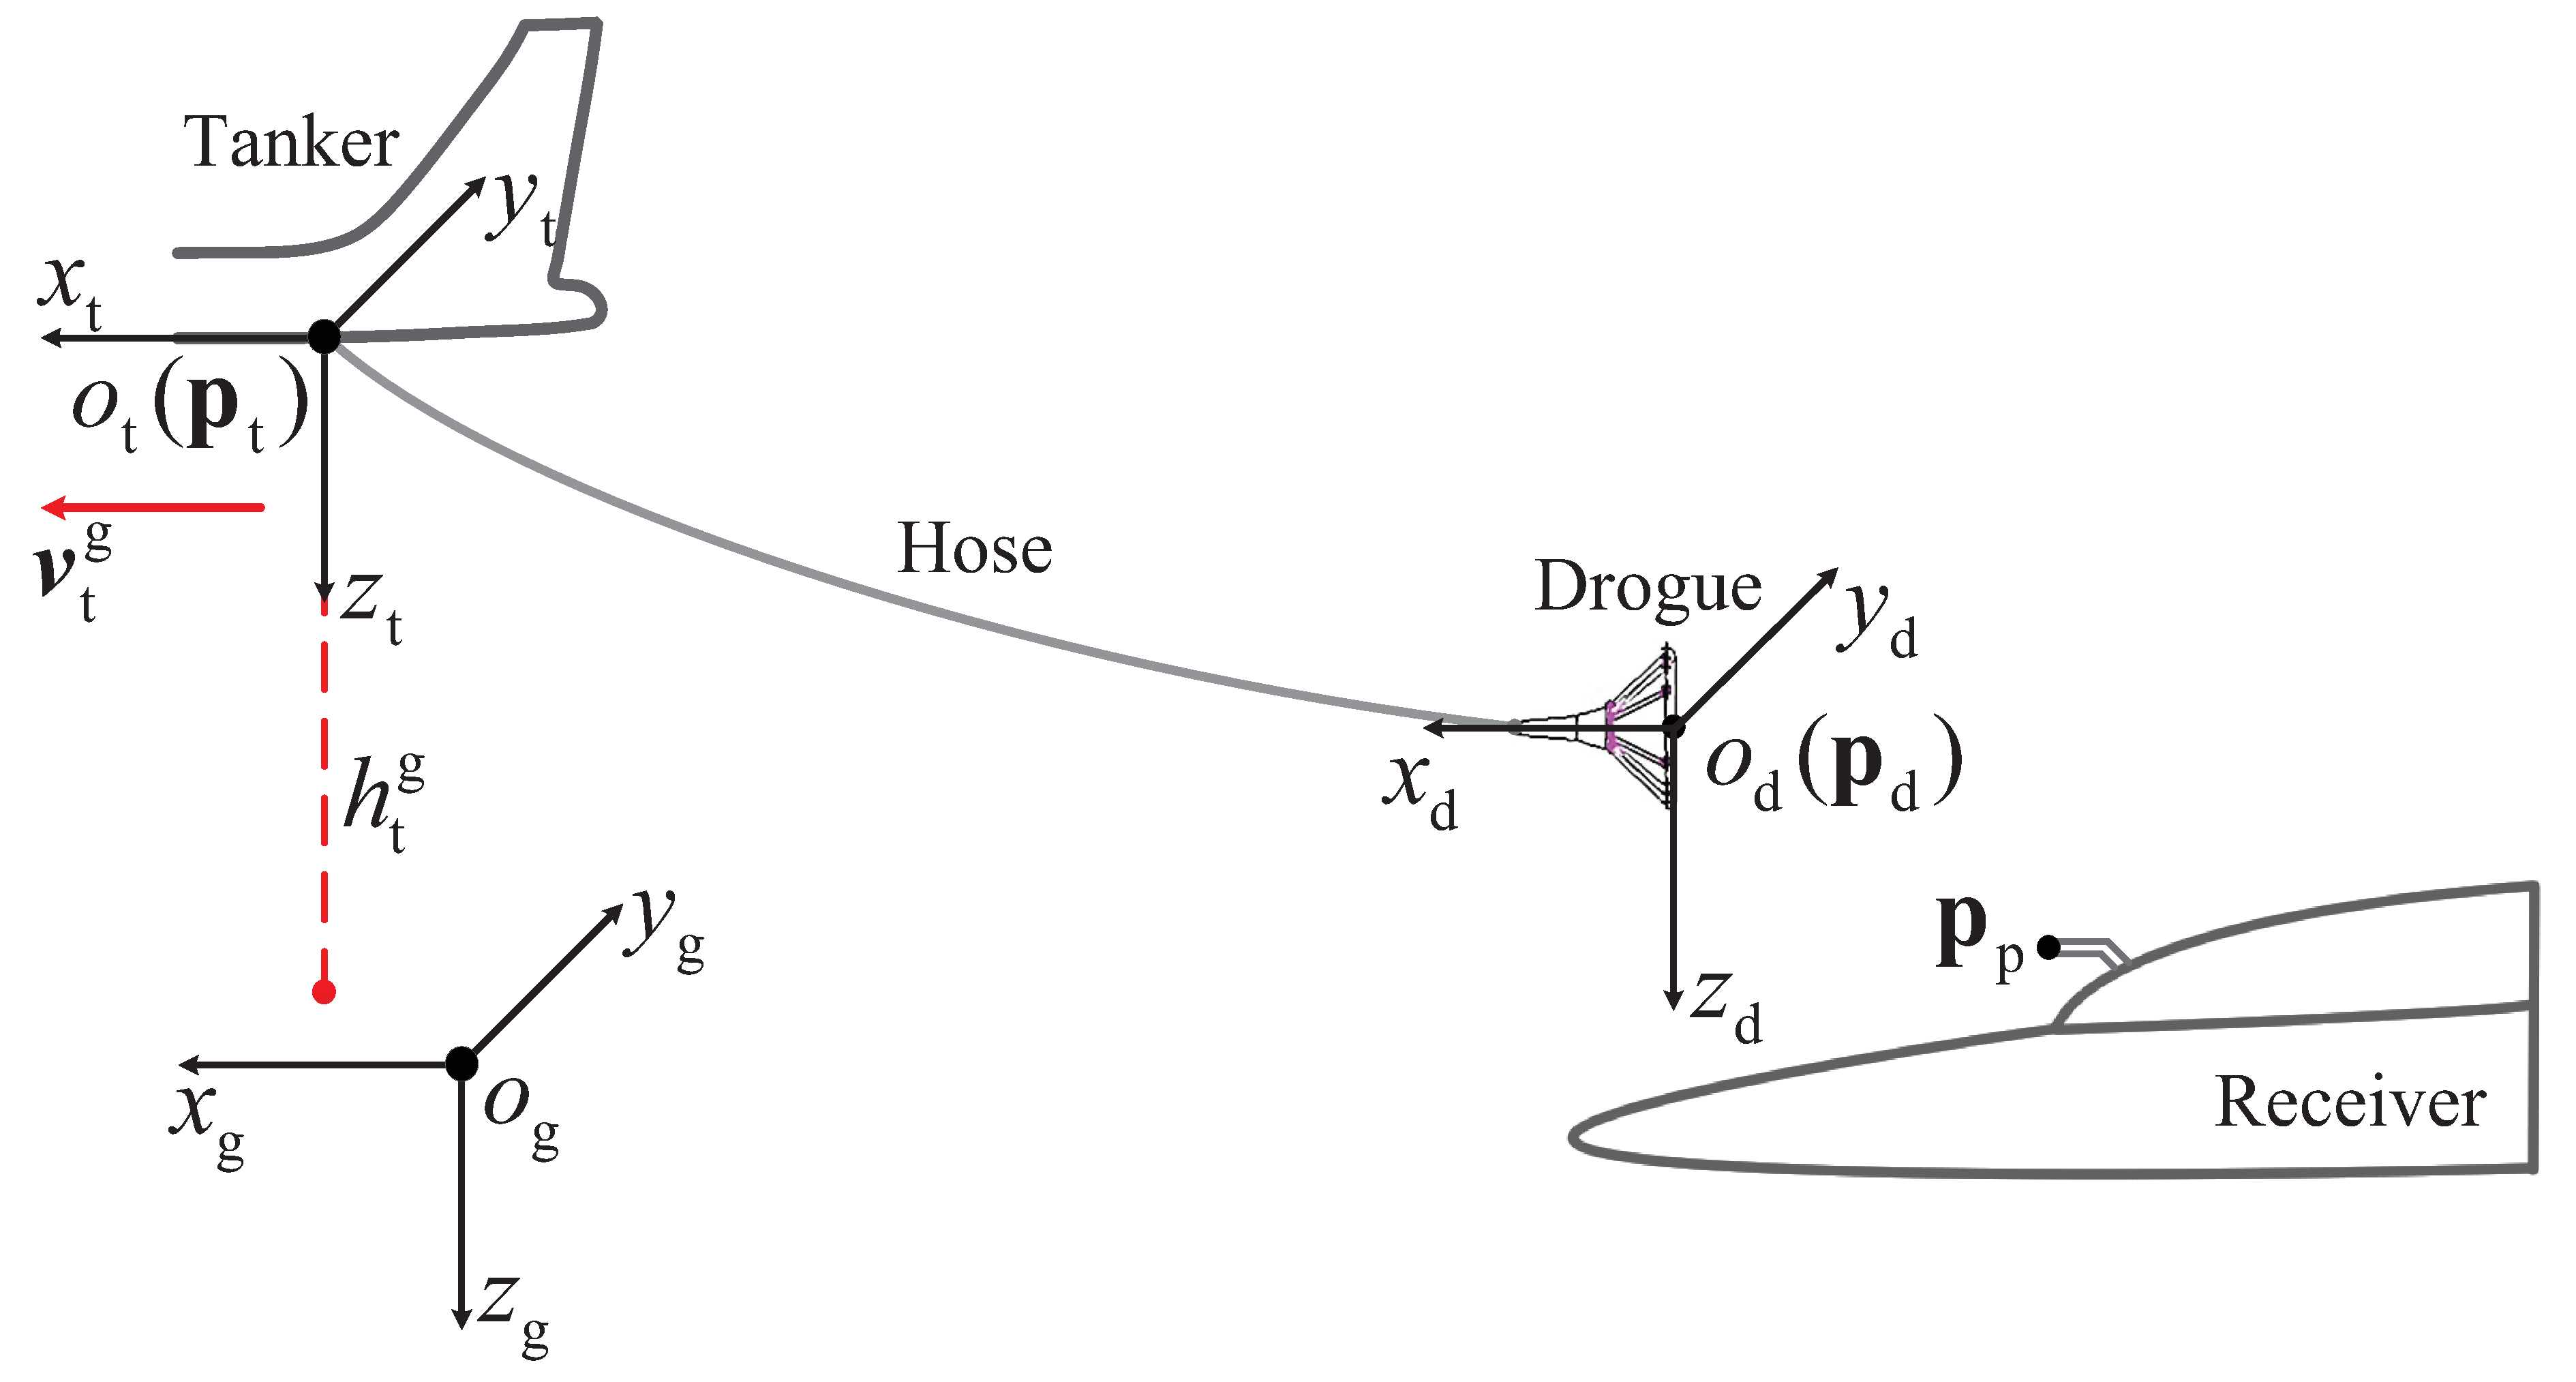
\includegraphics[
		width=10cm]{Figures/Figs_Ch7/Fig_Frames.eps}
	\end{center}
	\caption{Coordinate frames for the PDR system.}
	\label{Fig_Frames}
\end{figure}

\subsubsection{Variable mass receiver model}

The complexity of the receiver system
would make the system modelling difficult. To facilitate the derivation of
the dynamics equations including the effect of fuel transfer, the following
assumptions are introduced.

\textbf{Assumption 1.} A receiver system comprises two parts: a solid main
part and fuel tanks. The solid part is considered to be rigid, and the total
change of mass and inertial moment of the receiver is caused by that of fuel
tanks.

\textbf{Assumption 2. }The solid part is symmetric about the plane $o_{\text{%
		r}}x_{\text{r}}z_{\text{r}}$. Not only the geometric shape but also the mass
distribution are symmetric.

\textbf{Assumption 3.} The mass only changes during the fuel transfer.

\textbf{Assumption 4. }The receiver has $k$ fuel tanks. The tank position
and fuel mass distribution are symmetric about the plane $o_{\text{r}}x_{%
	\text{r}}z_{\text{r}}$. The mass of fuel in the $j$th tank is $%
m_{j},j=1,2,\cdots ,k$, and the distance vector $\mathbf{r}_{j}$ from its
mass center $o_{j}$ to the mass center of the receiver body $o_{\text{r}}$
is constant.

Based on these assumptions, the six-degree-of-freedom variable mass receiver
model (F-16 aircraft is considered) \cite{wang2016modeling} including dynamic
equations and kinematic equations is given as below. First, some variable
definitions are given. $\mathbf{p}_{\text{r}}=\left[
\begin{array}{ccc}
x_{\text{r}} & y_{\text{r}} & h_{\text{r}}%
\end{array}%
\right] ^{\text{T}}$ denotes the receiver position in the tanker frame with $%
x_{\text{r}}$ for the $x$-axis position value, $y_{\text{r}}$ for the $y$%
-axis position value, and $h_{\text{r}}$ for the $z$-axis height value. $%
\mathbf{v}_{\text{r}}=\left[
\begin{array}{ccc}
u_{\text{r}} & v_{\text{r}} & w_{\text{r}}%
\end{array}%
\right] ^{\text{T}}$ denotes the receiver velocity in the tanker frame with $%
u_{\text{r}}$ for the $x$-axis velocity value, $v_{\text{r}}$ for the $y$%
-axis velocity value, and $w_{\text{r}}$ for the $z$-axis velocity value. $%
\boldsymbol{\Theta }_{\text{r}}=\left[
\begin{array}{ccc}
\phi & \theta & \psi%
\end{array}%
\right] ^{\text{T}}$ denotes the receiver attitude angle with $\phi $ for
the roll angle, $\theta $ for the pitch angle, and $\psi $ for the yaw
angle. $\boldsymbol{\omega }_{\text{r}}=\left[
\begin{array}{ccc}
p & q & r%
\end{array}%
\right] ^{\text{T}}$ denotes the receiver body angular velocity with $p$ for
the roll rate, $q$ for the pitch rate, and $r$ for the yaw rate. The control
input for the receiver is $\mathbf{u}_{\text{r}}=\left[
\begin{array}{cccc}
\delta _{t} & \delta _{e} & \delta _{a} & \delta _{r}%
\end{array}%
\right] ^{\text{T}}$ with $\delta _{t}$, $\delta _{e}$, $\delta _{a}$ and $%
\delta _{r}$ denoting the thrust input and three control surface deflections
of the elevator, the aileron, and the rudder, respectively.

Translational dynamic equations:%
\begin{eqnarray}
\dot{u}_{\text{r}} &=&rv_{\text{r}}-qw_{\text{r}}-g\sin \theta +\frac{1}{m}%
\left( \bar{X}+F_{\text{T}}\right) -\frac{\dot{m}u_{\text{r}}}{m}  \notag \\
\dot{v}_{\text{r}} &=&pw_{\text{r}}-ru_{\text{r}}+g\sin \phi \cos \theta +%
\frac{1}{m}\bar{Y}-\frac{\dot{m}v_{\text{r}}}{m}  \label{Eq_TDE} \\
\dot{w}_{\text{r}} &=&qu_{\text{r}}-pv_{\text{r}}-g\cos \phi \cos \theta +%
\frac{1}{m}\bar{Z}-\frac{\dot{m}w_{\text{r}}}{m}.  \notag
\end{eqnarray}

Rotational dynamic equations:%
\begin{eqnarray}
\dot{p} &=&\left( c_{1}r+c_{2}p\right) q+c_{3}\bar{L}+c_{4}\left( \bar{N}+h_{%
	\text{E}}q\right) +\kappa _{1}p+\kappa _{2}r  \notag \\
\dot{q} &=&c_{5}pr-c_{6}\left( p^{2}-r^{2}\right) +c_{7}\left( \bar{M}-h_{%
	\text{E}}r\right) +\kappa _{3}q  \label{Eq_RDE} \\
\dot{r} &=&\left( c_{8}p-c_{2}r\right) q+c_{4}\bar{L}+c_{9}\left( \bar{N}+h_{%
	\text{E}}q\right) +\kappa _{4}p+\kappa _{5}r.  \notag
\end{eqnarray}

Rotational kinematical equations:%
\begin{eqnarray}
\dot{\phi} &=&p+\tan \theta \left( q\sin \phi +r\cos \phi \right)  \notag \\
\dot{\theta} &=&q\cos \phi -r\sin \phi  \label{Eq_RKE} \\
\dot{\psi} &=&\frac{q\sin \phi +r\cos \phi }{\cos \theta }.  \notag
\end{eqnarray}

Translational kinematical equations:%
\begin{eqnarray}
\dot{x}_{\text{r}} &=&u_{\text{r}}\cos \psi \cos \theta +v_{\text{r}}\left(
\cos \psi \sin \theta \sin \phi -\sin \psi \cos \phi \right)  \notag \\
&&+w_{\text{r}}\left( \cos \psi \sin \theta \cos \phi +\sin \psi \sin \phi
\right)  \notag \\
\dot{y}_{\text{r}} &=&u_{\text{r}}\sin \psi \cos \theta +v_{\text{r}}\left(
\sin \psi \sin \theta \sin \phi -\cos \psi \cos \phi \right)  \label{Eq_TKE}
\\
&&+w_{\text{r}}\left( \sin \psi \sin \theta \cos \phi +\cos \psi \sin \theta
\right)  \notag \\
\dot{h}_{\text{r}} &=&u_{\text{r}}\sin \theta -v_{\text{r}}\cos \theta \sin
\phi -w_{\text{r}}\cos \theta \cos \phi  \notag.
\end{eqnarray}%
Please refer to \cite{Waishek2009Derivation} for the detailed derivation
process. The definition and expression of other parameters in the above
equations are given in \textit{Appendix A}. The translational dynamic
equations (\ref{Eq_TDE}) and the rotational dynamic equations (\ref{Eq_RDE})
are different from their constant mass counterparts, while the rotational
kinematical equations (\ref{Eq_RKE}) and the translational kinematical
equations (\ref{Eq_TKE}) are the same as their constant mass counterparts.
Concretely, the change of mass has an effect on the translational dynamic
equations (\ref{Eq_TDE}), and the change of the inertia moment has an effect
on the rotational dynamic equations (\ref{Eq_RDE}).

In the tanker frame, the variable mass receiver model consisting of (\ref%
{Eq_TDE}), (\ref{Eq_RDE}), (\ref{Eq_RKE}), (\ref{Eq_TKE}) can be represented
by a compact form
\begin{equation}
\mathbf{\dot{x}}_{\text{r}}=\mathbf{f}\left( \mathbf{x}_{\text{r}},\mathbf{u}%
_{\text{r}},\mathbf{d}\right)  \label{Eq_LumpedModel}
\end{equation}%
where the state vector $\mathbf{x}_{\text{r}}=\left[
\begin{array}{cccccccccccc}
x_{\text{r}} & y_{\text{r}} & h_{\text{r}} & \phi & \theta & \psi & u_{\text{%
		r}} & v_{\text{r}} & w_{\text{r}} & p & q & r%
\end{array}%
\right] ^{\text{T}}$, the input vector $\mathbf{u}_{\text{r}}=\left[
\begin{array}{cccc}
\delta _{t} & \delta _{e} & \delta _{a} & \delta _{r}%
\end{array}%
\right] ^{\text{T}}$, $\mathbf{d}$ denotes various aerodynamic disturbances
including the atmospheric turbulence and the tanker vortex.

\subsection{Problem statement}

Suppose that, in the level and forward flight, $u_{\text{r}}=v_{\text{r}}=w_{%
	\text{r}}=p=q=r=0$. Under this trim condition, the trimmed state and trimmed
input are $\mathbf{x}_{\text{r}}^{\ast }$ and $\mathbf{u}_{\text{r}}^{\ast }$%
, which satisfy%
\begin{equation}
\mathbf{\dot{x}}_{\text{r}}^{\ast }=\mathbf{f}\left( \mathbf{x}_{\text{r}%
}^{\ast },\mathbf{u}_{\text{r}}^{\ast }\right).  \label{Eq_TrimedModel}
\end{equation}%
By defining the disturbed state and disturbed input as $\mathbf{\tilde{x}}_{%
	\text{r}}=\mathbf{x}_{\text{r}}-\mathbf{x}_{\text{r}}^{\ast },$ $\mathbf{%
	\tilde{u}}_{\text{r}}=\mathbf{u}_{\text{r}}-\mathbf{u}_{\text{r}}^{\ast },$
the disturbed system can be written as%
\begin{equation}
\begin{array}{l}
\mathbf{\dot{\tilde{x}}}_{\text{r}}=\mathbf{A\tilde{x}}_{\text{r}}+\mathbf{B%
	\tilde{u}}_{\text{r}}+\mathbf{g}\left( \mathbf{\tilde{x}}_{\text{r}}\right) +%
\mathbf{d}\left( \mathbf{\tilde{x}}_{\text{r}},\mathbf{\tilde{u}}_{\text{r}%
}\right) \\
\mathbf{\tilde{y}}_{\text{r}}=\mathbf{C\tilde{x}}_{\text{r}},\mathbf{\tilde{x%
}}_{\text{r}}\left( 0\right) =\mathbf{\tilde{x}}_{\text{r0}}%
\end{array}
\label{Eq_DisturbedModel}
\end{equation}%
where $\mathbf{A\triangleq }\left. \frac{\partial \mathbf{f}\left( \mathbf{x}%
	_{\text{r}},\mathbf{u}_{\text{r}}\right) }{\partial \mathbf{x}_{\text{r}}}%
\right\vert _{\mathbf{x}_{\text{r}}=\mathbf{x}_{\text{r}}^{\ast },\mathbf{u}%
	_{\text{r}}=\mathbf{u}_{\text{r}}^{\ast }}$, $\mathbf{B\triangleq }\left.
\frac{\partial \mathbf{f}\left( \mathbf{x}_{\text{r}},\mathbf{u}_{\text{r}%
	}\right) }{\partial \mathbf{u}_{\text{r}}}\right\vert _{\mathbf{x}_{\text{r}%
	}=\mathbf{x}_{\text{r}}^{\ast },\mathbf{u}_{\text{r}}=\mathbf{u}_{\text{r}%
	}^{\ast }}$, $\mathbf{g}\left( \mathbf{\tilde{x}}_{\text{r}}\right) $
denotes nonlinear terms, and $\mathbf{d}\left( \mathbf{\tilde{x}}_{\text{r}},%
\mathbf{\tilde{u}}_{\text{r}}\right) $ includes unmodelled dynamics and
disturbances. The output matrix $\mathbf{C\in
	%TCIMACRO{\U{211d} }%
	%BeginExpansion
	\mathbb{R}
	%EndExpansion
}^{3\times 12}$, and $\mathbf{\tilde{y}}_{\text{r}}=\mathbf{p}_{\text{r}}-%
\mathbf{p}_{\text{r}}^{\text{*}}$ with $\mathbf{p}_{\text{r}}^{\text{*}}$
for the trimmed position. $\mathbf{\tilde{x}}_{\text{r0}}\mathbf{\in
	%TCIMACRO{\U{211d} }%
	%BeginExpansion
	\mathbb{R}
	%EndExpansion
}^{12}$ is the initial state value.

\textbf{Control objective:} Design a station keeping controller $\mathbf{u}_{%
	\text{r}}$ for the receiver system (\ref{Eq_LumpedModel}) such that $\mathbf{%
	p}_{\text{r}}\left( t\right) -\mathbf{p}_{\text{r}}^{\text{d}}\left(
t\right) \rightarrow $ $\mathbf{0}$ or ${\mathbf{p}_{\text{r}}\left(
	t\right) -}\mathbf{p}_{\text{r}}^{\text{d}}\left( t\right) \rightarrow
\mathcal{B}\left( \mathbf{0}_{3\times 1},\delta \right) $) \footnote{$%
	\mathcal{B}\left( \mathbf{o},\delta \right) \triangleq \left\{ \boldsymbol{%
		\xi }\in
	%TCIMACRO{\U{211d} }%
	%BeginExpansion
	\mathbb{R}
	%EndExpansion
	^{3}\left\vert \left\Vert \boldsymbol{\xi }-\mathbf{o}\right\Vert \leq
	\delta \right. \right\} ,$ and the notation $\mathbf{x}\left( t\right)
	\rightarrow \mathcal{B}\left( \mathbf{o},\delta \right) $ means $\underset{%
		\mathbf{y}\in \mathcal{B}\left( \mathbf{o},\delta \right) }{\min }$ $%
	\left\Vert \mathbf{x}\left( t\right) -\mathbf{y}\right\Vert \rightarrow 0.$}
as $t\rightarrow \infty $, $\delta \in
%TCIMACRO{\U{211d} }%
%BeginExpansion
\mathbb{R}
%EndExpansion
_{+}\cup \left\{ 0\right\} $. Equivalently, design a tracking controller $%
\mathbf{u}_{\text{r}}$ for the system (\ref{Eq_DisturbedModel}) such that $%
\mathbf{\tilde{y}}_{\text{r}}\left( t\right) -\mathbf{\tilde{y}}_{\text{r}}^{%
	\text{d}}\left( t\right) \rightarrow $ $\mathbf{0}$ or $\mathbf{\tilde{y}}_{%
	\text{r}}{\left( t\right) -}\mathbf{\tilde{y}}_{\text{r}}^{\text{d}}\left(
t\right) \rightarrow \mathcal{B}\left( \mathbf{0}_{3\times 1},\delta \right)
$ as $t\rightarrow \infty $ when there exist disturbances, where $\mathbf{p}%
_{\text{r}}^{\text{d}}$ is the reference trajectory, $\mathbf{\tilde{y}}_{%
	\text{r}}^{\text{d}}=\mathbf{p}_{\text{r}}^{\text{d}}-\mathbf{p}_{\text{r}}^{%
	\text{*}}$ is the disturbed reference trajectory.

The system (\ref{Eq_DisturbedModel}) is a multi-input multi-output (MIMO)
nonlinear system with nonminimum-phase, multi-disturbance, and variable-mass
features. Thus, the latter control design needs to deal with nonlinearity,
uncertainty, and disturbances simultaneously. ASD-based control can provide
an effective solution to this problem.

\section{ASD-based Station-keeping Controller Design}

\label{ASDBC}

This section presents the station-keeping controller design. First, based on
additive state decomposition, the considered system (\ref{Eq_DisturbedModel}%
) is decomposed into two subsystems: an LTI primary system (\ref{sys_pri})
including all disturbances and a deterministic nonlinear secondary system (%
\ref{sys_sec}). Correspondingly, the original tracking task for system (\ref%
{Eq_DisturbedModel}) is decomposed into two subtasks: a tracking subtask for
(\ref{sys_pri}) and a stabilization subtask for (\ref{sys_sec}).

\subsection{Basic control idea}

Conventionally, most station-keeping controllers are designed by using
control methods for linear systems after linearizing the nonlinear receiver
system directly, as shown in Fig.~\ref{Fig_ControlIdea}(a). However,
abandoning the nonlinear term directly may limit the control effect and make
the final closed-loop system fragile to system perturbation and external
disturbances. If the nonlinearity information of the nonlinear receiver
system can be considered properly, better control effect would be expected.
Thus, in this chapter, a new control idea displayed in Fig.~\ref%
{Fig_ControlIdea}(b) is proposed. Based on ASD, we aim to consider the
nonlinear part of the receiver system in the secondary system. Then, the
primary system from the input $\mathbf{u}_{\text{p}}$ to the state $\mathbf{x%
}_{\text{p}}$ is an LTI system, which can still adopt the conventional
station-keeping controller. The closed-loop system of the secondary system
can be realized by a computer, and the primary system ($B-C$) can be
obtained by subtracting the complementary secondary system ($C$) from the
original system ($A$).
\begin{figure}[tph]
	\begin{center}
		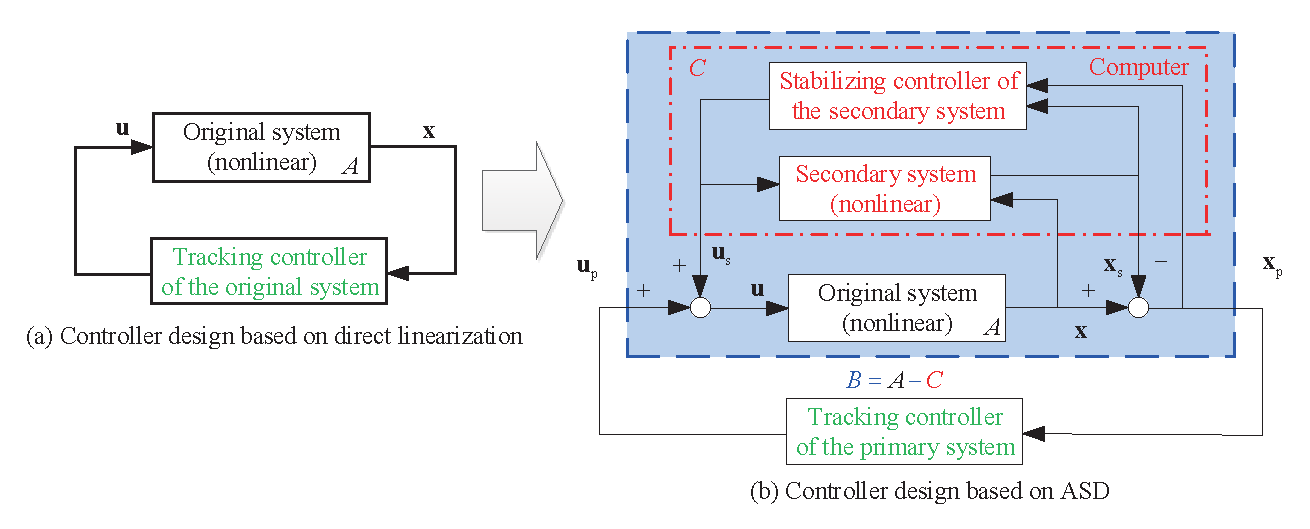
\includegraphics[
		scale=0.6]{Figures/Figs_Ch7/Fig_ControlIdea.eps}
	\end{center}
	\caption{Two control ideas.}
	\label{Fig_ControlIdea}
\end{figure}

\subsection{Additive state decomposition}

Additive state decomposition (ASD) \cite{quan2015additive} is a
decomposition method for nonlinear systems just like superposition principle
for linear systems. In the following,
ASD is introduced to decompose the aforementioned receiver model into two
subsystems to make the following controller design more flexible and easier.

Consider system (\ref{Eq_DisturbedModel}) as the original system. By
applying ASD, the primary system is chosen as%
\begin{equation}
\begin{array}{l}
\mathbf{\dot{\tilde{x}}}_{\text{r,p}}=\mathbf{A\tilde{x}}_{\text{r,p}}+%
\mathbf{B\tilde{u}}_{\text{r,p}}+\mathbf{d}\left( \mathbf{\tilde{x}}_{\text{r%
}},\mathbf{\tilde{u}}_{\text{r}}\right) \\
\mathbf{\tilde{y}}_{\text{r,p}}=\mathbf{C\tilde{x}}_{\text{r,p}},\mathbf{%
	\tilde{x}}_{\text{r,p}}\left( 0\right) =\mathbf{\tilde{x}}_{\text{r0}}.%
\end{array}
\label{equ_pri}
\end{equation}%
Then, subtracting the primary system (\ref{equ_pri}) from the original
system (\ref{Eq_DisturbedModel}) gives%
\begin{equation}
\begin{array}{l}
\mathbf{\dot{\tilde{x}}}_{\text{r}}-\mathbf{\dot{\tilde{x}}}_{\text{r,p}}=%
\mathbf{A}\left( \mathbf{\tilde{x}}_{\text{r}}-\mathbf{\tilde{x}}_{\text{r,p}%
}\right) +\mathbf{B}\left( \mathbf{\tilde{u}}_{\text{r}}-\mathbf{\tilde{u}}_{%
	\text{r,p}}\right) +\mathbf{g}\left( \mathbf{\tilde{x}}_{\text{r}}\right) \\
\mathbf{\tilde{y}}_{\text{r}}-\mathbf{\tilde{y}}_{\text{r,p}}=\mathbf{C}%
\left( \mathbf{\tilde{x}}_{\text{r}}-\mathbf{\tilde{x}}_{\text{r,p}}\right) ,%
\mathbf{\tilde{x}}_{\text{r}}\left( 0\right) -\mathbf{\tilde{x}}_{\text{r,p}%
}\left( 0\right) =\mathbf{0}.%
\end{array}
\label{equ_sec}
\end{equation}%
Next, by defining
\begin{equation}
\mathbf{\tilde{x}}_{\text{r,s}}=\mathbf{\tilde{x}}_{\text{r}}-\mathbf{\tilde{%
		x}}_{\text{r,p}},\text{ }\mathbf{\tilde{y}}_{\text{r,s}}=\mathbf{\tilde{y}}_{%
	\text{r}}-\mathbf{\tilde{y}}_{\text{r,p}},\text{ }\mathbf{\tilde{u}}_{\text{%
		r,s}}=\mathbf{\tilde{u}}_{\text{r}}-\mathbf{\tilde{u}}_{\text{r,p}}
\label{relation}
\end{equation}%
system (\ref{equ_pri}) and system (\ref{equ_sec}) become%
\begin{align}
\text{Primary system}& \text{:}\left\{
\begin{array}{l}
\mathbf{\dot{\tilde{x}}}_{\text{r,p}}=\mathbf{A\tilde{x}}_{\text{r,p}}+%
\mathbf{B\tilde{u}}_{\text{r,p}}+\mathbf{d}\left( \mathbf{\tilde{x}}_{\text{%
		r,s}}+\mathbf{\tilde{x}}_{\text{r,p}},\mathbf{\tilde{u}}_{\text{r,p}}+%
\mathbf{\tilde{u}}_{\text{r,s}}\right) \\
\mathbf{\tilde{y}}_{\text{r,p}}=\mathbf{C\tilde{x}}_{\text{r,p}},\mathbf{%
	\tilde{x}}_{\text{r,p}}\left( 0\right) =\mathbf{\tilde{x}}_{\text{r0}}%
\end{array}%
\right.  \label{sys_pri} \\
\text{Secondary system}& \text{:}\left\{
\begin{array}{l}
\mathbf{\dot{\tilde{x}}}_{\text{r,s}}=\mathbf{A\tilde{x}}_{\text{r,s}}+%
\mathbf{B\tilde{u}}_{\text{r,s}}+\mathbf{g}\left( \mathbf{\tilde{x}}_{\text{%
		r,s}}+\mathbf{\tilde{x}}_{\text{r,p}}\right) \\
\mathbf{\tilde{y}}_{\text{r,s}}=\mathbf{C\tilde{x}}_{\text{r,s}},\mathbf{%
	\tilde{x}}_{\text{r,s}}\left( 0\right) =\mathbf{0}.%
\end{array}%
\right.   \label{sys_sec}
\end{align}%
The two decomposed systems have the same dimensions with the original system
(\ref{Eq_DisturbedModel}). Conversely, the original system (\ref%
{Eq_DisturbedModel}) can be replaced by putting the primary system (\ref%
{sys_pri}) and the secondary system (\ref{sys_sec}) together, which means
the state and the output satisfy%
\begin{equation}
\mathbf{\tilde{x}}_{\text{r}}=\mathbf{\tilde{x}}_{\text{r,s}}+\mathbf{\tilde{%
		x}}_{\text{r,p}},\text{ }\mathbf{\tilde{y}}_{\text{r}}=\mathbf{\tilde{y}}_{%
	\text{r,s}}+\mathbf{\tilde{y}}_{\text{r,p}},\text{ }\mathbf{\tilde{u}}_{%
	\text{r}}=\mathbf{\tilde{u}}_{\text{r,s}}+\mathbf{\tilde{u}}_{\text{r,p}}.
\label{equ_relation}
\end{equation}

It is clear from equations (\ref{sys_pri})-(\ref{equ_relation}) that if the
controller $\mathbf{\tilde{u}}_{\text{r,p}}$ drives $\mathbf{\tilde{y}}_{%
	\text{r,p}}\left( t\right) -\mathbf{\tilde{y}}_{\text{r}}^{\text{d}}\left(
t\right) \rightarrow $ $\mathbf{0}$ or $\mathbf{\tilde{y}}_{\text{r,p}}{%
	\left( t\right) -}\mathbf{\tilde{y}}_{\text{r}}^{\text{d}}\left( t\right)
\rightarrow \mathcal{B}\left( \mathbf{0}_{3\times 1},\delta \right) $ as $%
t\rightarrow \infty $ and the controller $\mathbf{\tilde{u}}_{\text{r,s}}$
drives $\mathbf{\tilde{x}}_{\text{r,s}}\left( t\right)\rightarrow \mathbf{0}$ as $%
t\rightarrow \infty ,$ then $\mathbf{\tilde{y}}_{\text{r}}\left( t\right) -%
\mathbf{\tilde{y}}_{\text{r}}^{\text{d}}\left( t\right) \rightarrow $ $%
\mathbf{0}$ or $\mathbf{\tilde{y}}_{\text{r}}{\left( t\right) -}\mathbf{%
	\tilde{y}}_{\text{r}}^{\text{d}}\left( t\right) \rightarrow \mathcal{B}%
\left( \mathbf{0}_{3\times 1},\delta \right) $ as $t\rightarrow \infty $.
The strategy here is to assign the tracking subtask to the primary system (%
\ref{sys_pri}) and the stabilization subtask to the secondary system (\ref%
{sys_sec}), which is shown in Fig.~\ref{Fig_ASD}. Since system (\ref{sys_pri}%
) is an LTI system including all disturbances, standard design methods in
either frequency domain or time domain, such as the PI control method, can
be used to handle the tracking problem. On the other hand, system (\ref%
{sys_sec}) is a deterministic nonlinear system, many nonlinear stabilizing
control methods can be applied to solve the stabilization problem. It should
be noticed that the ASD offers a two-degree-of-freedom way to tackle a
tracking task under disturbances and a nonlinear stabilization task
respectively, which reduces the difficulty of the original problem. The primary controller designed for the tracking task and the secondary controller designed for the nonlinear stabilization task can be viewed as two one-degree-of-freedom controllers. The final two-degree-of-freedom controller can be obtained by combining the primary controller and the secondary controller.
\begin{figure}[tph]
	\begin{center}
		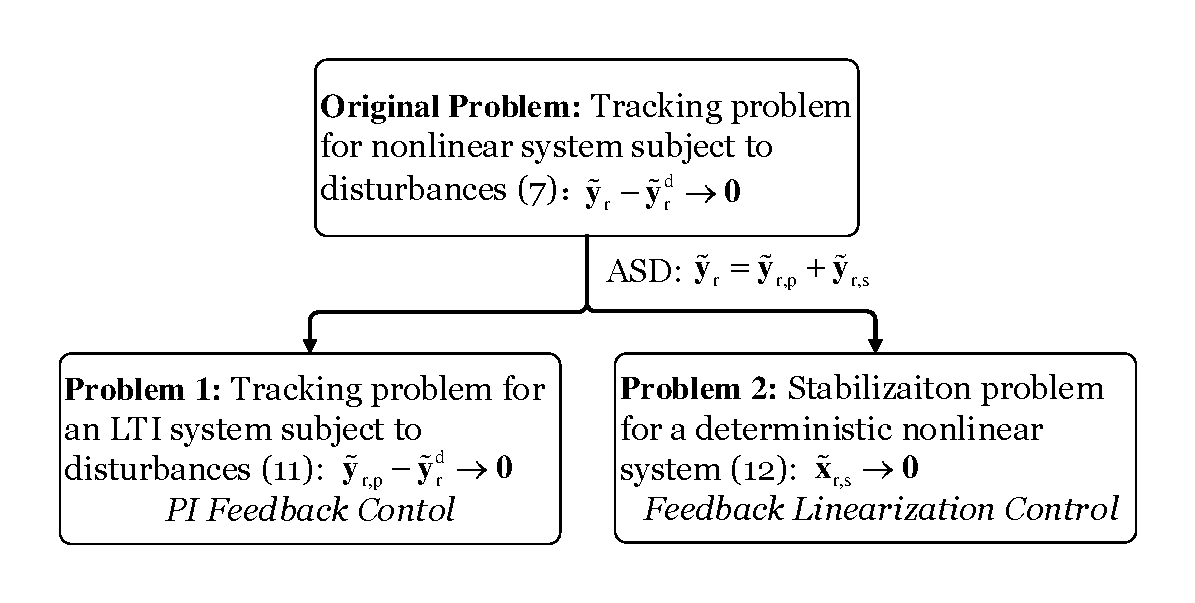
\includegraphics[
		width=12cm]{Figures/Figs_Ch7/Fig_ASD.eps}
	\end{center}
	\caption{Additive state decomposition of system (\protect\ref%
		{Eq_DisturbedModel}).}
	\label{Fig_ASD}
\end{figure}

\subsection{Controller design for the primary and secondary systems}

So far, the considered system has been decomposed into two subsystems in
charge of corresponding subtasks. In this section, the controller design is
investigated in the form of two problems with respect to two subtasks,
respectively. Because the system dimension of the receiver is high,
controllers are often designed for the decoupled longitudinal channel and
lateral channel respectively. In the following, the controller design for
the longitudinal channel is taken into consideration for an illustration (a
subscript `lon' is added to every variable in the following, while `lat'
stands for the lateral channel). The control idea and design process of the
lateral channel is similar, and thus omitted here. The longitudinal channel
has the state $\mathbf{x}_{\text{rlon}}=\left[
\begin{array}{cccccc}
x_{\text{r}} & h_{\text{r}} & \theta & V_{\text{r}} & \alpha & q%
\end{array}%
\right] ^{\text{T}}$ and the input $\mathbf{u}_{\text{rlon}}=\left[
\begin{array}{cc}
\delta _{t} & \delta _{e}%
\end{array}%
\right] ^{\text{T}}$, while the lateral channel has the state $\mathbf{x}_{%
	\text{rlat}}=\left[
\begin{array}{cccccc}
y_{\text{r}} & \psi & \phi & \beta & p & r%
\end{array}%
\right] ^{\text{T}}$ and the input $\mathbf{u}_{\text{rlat}}=\left[
\begin{array}{cc}
\delta _{a} & \delta _{r}%
\end{array}%
\right] ^{\text{T}}$.

\subsubsection{Problem 1. Tracking problem}

For (\ref{sys_pri}), design a PI tracking controller%
\begin{equation}
\mathbf{\tilde{u}}_{\text{rlon,p}}=\mathbf{\tilde{u}}_{\text{rlon,p}}\left(
\mathbf{\tilde{x}}_{\text{rlon,p}},\int_{0}^{t}\left( \mathbf{\tilde{y}}_{%
	\text{rlon,p}}\left( s\right) -\mathbf{\tilde{y}}_{\text{rlon}}^{\text{d}%
}\left( s\right) \right) \text{d}s\right)  \label{Ctr_Primary0}
\end{equation}%
such that $\mathbf{e}_{\text{rlon,p}}=\mathbf{\tilde{y}}_{\text{rlon,p}%
}\left( t\right) -\mathbf{\tilde{y}}_{\text{rlon}}^{\text{d}}\left( t\right)
\rightarrow \mathbf{0}$ as $t\rightarrow \infty $, meanwhile keeping $%
\mathbf{\tilde{x}}_{\text{rlon,p}}$ bounded.

Intuitively, to remove the tracking error, an integral action must be
employed in the controller%
\begin{equation}
\mathbf{q}_{\text{rlon,p}}=\int_{0}^{t}\mathbf{e}_{\text{rlon,p}}\left(
s\right) \text{d}s=\int_{0}^{t}\left( \mathbf{\tilde{y}}_{\text{rlon,p}%
}\left( s\right) -\mathbf{\tilde{y}}_{\text{rlon}}^{\text{d}}\left( s\right)
\right) \text{d}s.  \label{Eq_Iterm}
\end{equation}%
By combining (\ref{sys_pri}) with (\ref{Eq_Iterm}), the manipulated
augmented system of (\ref{sys_pri}) is
\begin{equation*}
\left[
\begin{array}{c}
\mathbf{\dot{\tilde{x}}}_{\text{rlon,p}} \\
\mathbf{\dot{q}}_{\text{rlon,p}}%
\end{array}%
\right] =\left[
\begin{array}{cc}
\mathbf{A}_{\text{lon}} & \mathbf{0} \\
\mathbf{C}_{\text{lon}} & \mathbf{0}%
\end{array}%
\right] \left[
\begin{array}{c}
\mathbf{\tilde{x}}_{\text{rlon,p}} \\
\mathbf{q}_{\text{rlon,p}}%
\end{array}%
\right] +\left[
\begin{array}{c}
\mathbf{B}_{\text{lon}} \\
\mathbf{0}%
\end{array}%
\right] \mathbf{\tilde{u}}_{\text{rlon,p}}-\left[
\begin{array}{c}
\mathbf{0} \\
\mathbf{I}%
\end{array}%
\right] \mathbf{\tilde{y}}_{\text{rlon}}^{\text{d}}+\left[
\begin{array}{c}
\mathbf{I} \\
\mathbf{0}%
\end{array}%
\right] \mathbf{d}\left( \mathbf{\tilde{x}}_{\text{rlon}},\mathbf{\tilde{u}}%
_{\text{rlon}}\right).
\end{equation*}%
According to \cite{ogata2002modern}, a state feedback controller can be
designed as%
\begin{equation}
\mathbf{\tilde{u}}_{\text{rlon,p}}=-\mathbf{K}_{\mathbf{x}\text{lon}}\mathbf{%
	\tilde{x}}_{\text{rlon,p}}-\mathbf{K}_{\mathbf{e}\text{lon}}\mathbf{q}_{%
	\text{rlon,p}}
\end{equation}%
where $\mathbf{K}_{\mathbf{x}\text{lon}}\in
%TCIMACRO{\U{211d} }%
%BeginExpansion
\mathbb{R}
%EndExpansion
^{2\times 6},\mathbf{K}_{\mathbf{e}\text{lon}}\in
%TCIMACRO{\U{211d} }%
%BeginExpansion
\mathbb{R}
%EndExpansion
^{2\times 2}.$ The LQR method is utilized to determine the feedback matrices
$\mathbf{K}_{\mathbf{x}\text{lon}},\mathbf{K}_{\mathbf{e}\text{lon}},$ and
the cost function is%
\begin{equation*}
J\left( \mathbf{\tilde{u}}_{\text{rlon,p}}\right) =\underset{\mathbf{K}_{%
		\mathbf{x}\text{lon}},\mathbf{K}_{\mathbf{e}\text{lon}}}{\arg \min }%
\int_{0}^{\infty }\left\{ \left[
\begin{array}{cc}
\mathbf{\tilde{x}}_{\text{rlon,p}}^{\text{T}} & \mathbf{q}_{\text{rlon,p}}^{%
	\text{T}}%
\end{array}%
\right] \mathbf{Q}_{\text{rlon}}\left[
\begin{array}{c}
\mathbf{\tilde{x}}_{\text{rlon,p}} \\
\mathbf{q}_{\text{rlon,p}}%
\end{array}%
\right] +\mathbf{\tilde{u}}_{\text{rlon,p}}^{\text{T}}\mathbf{R_{\text{rlon}}%
	\tilde{u}}_{\text{rlon,p}}\right\} \text{d}t.
\end{equation*}%
The feedback matrices $\mathbf{K}_{\mathbf{x}\text{lon}},\mathbf{K}_{\mathbf{%
		e}\text{lon}}$ can be determined by choosing proper $\mathbf{Q}_{\text{rlon}%
} $ and $\mathbf{R}_{\text{rlon}}$\textbf{. }The structure of the
closed-loop primary system is displayed in Fig.~\ref{Fig_PController}.
\begin{figure}[tph]
	\begin{center}
		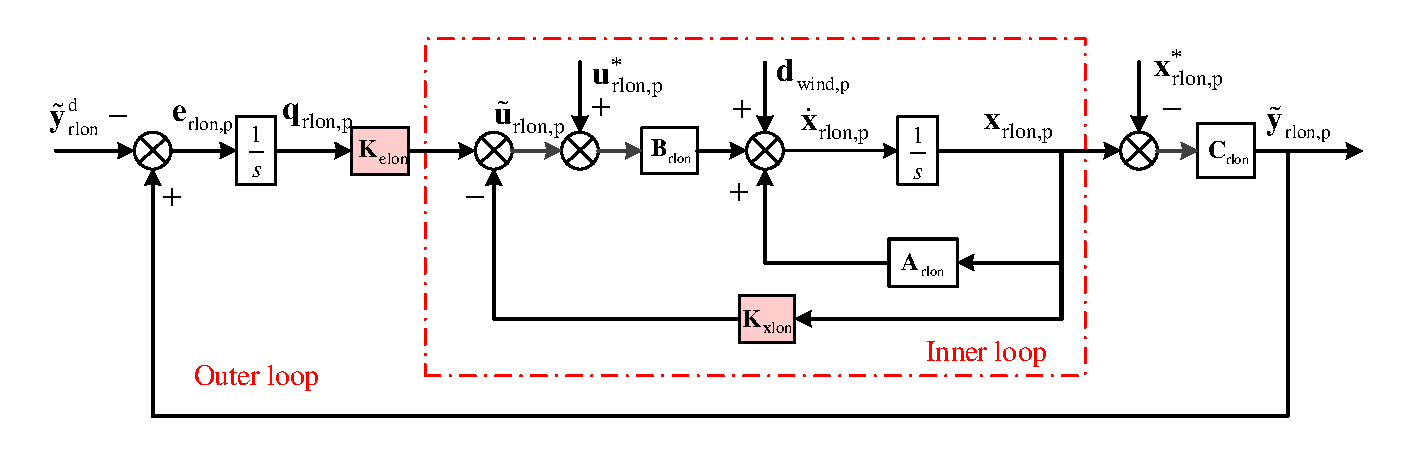
\includegraphics[
		width=12cm]{Figures/Figs_Ch7/Fig_PController.eps}
	\end{center}
	\caption{Closed-loop primary system.}
	\label{Fig_PController}
\end{figure}

\textbf{Theorem 1.} \textit{For system (\ref{sys_pri}), if the controller is
	designed as}%
\begin{equation}
\mathbf{\tilde{u}}_{\text{rlon,p}}=-\mathbf{K}_{\mathbf{x}\text{lon}}\mathbf{%
	\tilde{x}}_{\text{rlon,p}}-\mathbf{K}_{\mathbf{e}\text{lon}}\mathbf{q}_{%
	\text{rlon,p}}  \label{Ctr_Pri2}
\end{equation}%
\textit{\ then }$\mathbf{\tilde{y}}_{\text{rlon,p}}\left( t\right) -\mathbf{%
	\tilde{y}}_{\text{rlon}}^{\text{d}}\left( t\right) \rightarrow \mathbf{0}$%
\textit{\ as }$t\rightarrow \infty $, \textit{\ and }$\mathbf{\tilde{x}}_{%
	\text{rlon,p}}$\textit{\ is bounded. }

\textit{Proof. }See \cite{ogata2002modern}. $\square $

\subsubsection{Problem 2. Stabilization problem}

For (\ref{sys_sec}), design a stabilizing controller%
\begin{equation}
\mathbf{\tilde{u}}_{\text{rlon,s}}=\mathbf{\tilde{u}}_{\text{rlon,s}}\left(
\mathbf{\tilde{x}}_{\text{rlon,s}},\mathbf{\tilde{x}}_{\text{rlon,p}}\right)
\label{Ctr_Sec0}
\end{equation}%
such that $\mathbf{\tilde{x}}_{\text{rlon,s}}\left( t\right)\rightarrow \mathbf{0}$ as $%
t\rightarrow \infty $.

In the following, a feedback linearization controller will be designed. In order to
make the controller design easier, a virtual output variable is defined as
\begin{equation}
\mathbf{\bar{y}}_{\text{rlon,s}}=\mathbf{C}_{\text{slon}}\mathbf{\tilde{x}}_{%
	\text{rlon,s}}  \label{newoutput}
\end{equation}%
where $\mathbf{C}_{\text{slon}}\in
%TCIMACRO{\U{211d} }%
%BeginExpansion
\mathbb{R}
%EndExpansion
^{2\times 6}.$ If the new output matrix $\mathbf{C}_{\text{slon}}$ makes the
system from $\mathbf{\tilde{u}}_{\text{rlon,s}}$ to $\mathbf{\bar{y}}_{\text{%
		rlon,s}}$ be a minimum-phase system, then $\mathbf{\bar{y}}_{\text{rlon,s}%
}\rightarrow \mathbf{0}$ implies $\mathbf{\tilde{x}}_{\text{rlon,s}%
}\rightarrow \mathbf{0}$. A method for determining the output matrix $%
\mathbf{C}_{\text{slon}}$ is given in \cite{quan2015proportional}. After
obtaining feedback matrix $\mathbf{K}_{\mathbf{x}\text{lon}}$, $\mathbf{A}_{%
	\text{lon}}\mathbf{+B}_{\text{lon}}\mathbf{K}_{\mathbf{x}\text{lon}}$ is
stable. Thus, according to Lyapunov function, there exist $\mathbf{P}$ and $%
\mathbf{M}$ such that%
\begin{equation*}
\mathbf{P}\left( \mathbf{A}_{\text{lon}}\mathbf{+B}_{\text{lon}}\mathbf{K}_{%
	\mathbf{x}\text{lon}}\right) +\left( \mathbf{A}_{\text{lon}}\mathbf{+B}_{%
	\text{lon}}\mathbf{K}_{\mathbf{x}\text{lon}}\right) ^{\text{T}}\mathbf{P=-M}.
\end{equation*}%
Then, the output matrix $\mathbf{C}_{\text{slon}}$ can be determined as%
\begin{equation*}
\mathbf{C}_{\text{slon}}=\mathbf{PB}_{\text{lon}}\mathbf{.}
\end{equation*}%
Differentiating Eq.~(\ref{newoutput}), one has%
\begin{equation}
\mathbf{\dot{\bar{y}}}_{\text{rlon,s}}=\mathbf{C}_{\text{slon}}\mathbf{A}_{%
	\text{lon}}\mathbf{\tilde{x}}_{\text{rlon,s}}+\mathbf{C}_{\text{slon}}%
\mathbf{B}_{\text{lon}}\mathbf{\tilde{u}}_{\text{rlon,s}}+\mathbf{C}_{\text{%
		slon}}\mathbf{g}\left( \mathbf{\tilde{x}}_{\text{rlon,s}}+\mathbf{\tilde{x}}%
_{\text{rlon,p}}\right).
\end{equation}%
A control input can be designed as%
\begin{equation}
\mathbf{\tilde{u}}_{\text{rlon,s}}=\left( \mathbf{C}_{\text{slon}}\mathbf{B}%
_{\text{lon}}\right) ^{-1}\left( \mathbf{v}_{\text{rlon,s}}-\mathbf{C}_{%
	\text{slon}}\mathbf{A}_{\text{lon}}\mathbf{\tilde{x}}_{\text{rlon,s}}-%
\mathbf{C}_{\text{slon}}\mathbf{g}\left( \mathbf{\tilde{x}}_{\text{rlon,s}}+%
\mathbf{\tilde{x}}_{\text{rlon,p}}\right) \right)
\end{equation}%
where $\mathbf{v}_{\text{rlon,s}}$ is a virtual input. The choice of $%
\mathbf{C}_{\text{slon}}$ needs to make $\mathbf{C}_{\text{slon}}\mathbf{B}_{%
	\text{lon}}$ invertible. Then, it can be obtained
\begin{equation*}
\mathbf{\dot{\bar{y}}}_{\text{rlon,s}}=\mathbf{v}_{\text{rlon,s}}.
\end{equation*}%
Design
\begin{equation*}
\mathbf{v}_{\text{rlon,s}}=-\mathbf{K}_{\text{rlon}}\mathbf{\bar{y}}_{\text{%
		rlon,s}}
\end{equation*}%
where $\mathbf{K}_{\text{rlon}}\in
%TCIMACRO{\U{211d} }%
%BeginExpansion
\mathbb{R}
%EndExpansion
^{2\times 2}$ is the controller parameter. Then, one has%
\begin{equation*}
\mathbf{\dot{\bar{y}}}_{\text{rlon,s}}=-\mathbf{K}_{\text{rlon}}\mathbf{\bar{%
		y}}_{\text{rlon,s}}
\end{equation*}%
which can guarantee that $\mathbf{\bar{y}}_{\text{rlon,s}}\rightarrow
\mathbf{0}$ exponentially, and further can guarantee that $\mathbf{\tilde{x}}%
_{\text{rlon,s}}\rightarrow \mathbf{0}$ exponentially.

\textbf{Theorem 2.} \textit{For system (\ref{sys_sec}), if there exists a
	control input }%
\begin{equation}
\mathbf{\tilde{u}}_{\text{rlon,s}}=\left( \mathbf{C}_{\text{slon}}\mathbf{B}%
_{\text{lon}}\right) ^{-1}\left( -\mathbf{K}_{\text{rlon}}\mathbf{\bar{y}}_{%
	\text{rlon,s}}-\mathbf{C}_{\text{slon}}\mathbf{A}_{\text{lon}}\mathbf{\tilde{%
		x}}_{\text{rlon,s}}-\mathbf{C}_{\text{slon}}\mathbf{g}\left( \mathbf{\tilde{x%
}}_{\text{rlon,s}}+\mathbf{\tilde{x}}_{\text{rlon,p}}\right) \right)
\label{Ctr_sec0}
\end{equation}%
\textit{\ where }$\mathbf{K}_{\text{rlon}}\in
%TCIMACRO{\U{211d} }%
%BeginExpansion
\mathbb{R}
%EndExpansion
^{2\times 2}$ \textit{and} $\mathbf{C}_{\text{slon}}=\mathbf{PB}_{\text{lon}%
} $\textit{, such that}%
\begin{equation}
\mathbf{\dot{\bar{y}}}_{\text{rlon,s}}=-\mathbf{K}_{\text{rlon}}\mathbf{\bar{%
		y}}_{\text{rlon,s}}  \label{feedback-gain}
\end{equation}%
\textit{is stable, then }$\mathbf{\tilde{x}}_{\text{rlon,s}}\left( t\right)\rightarrow
\mathbf{0}$ as $t\rightarrow \infty $\textit{.}

\textit{Proof. }See \textit{\cite{quan2015proportional}}. $\square $

Controller design for the decomposed systems (\ref{sys_pri}) and (\ref%
{sys_sec}) requires their states and outputs as feedback variables. However,
they are virtual and unknown. For such a purpose, an observer is designed in
\emph{Theorem 3} to estimate $\mathbf{\tilde{x}}_{\text{rlon,p}}$, $\mathbf{%
	\tilde{x}}_{\text{rlon,s}}$ and $\mathbf{\tilde{y}}_{\text{rlon,p}}.$

\textbf{\textbf{Theorem 3}}.\textit{\ Suppose that an observer is designed
	to estimate }$\mathbf{\tilde{x}}_{\text{rlon,p}}$, $\mathbf{\tilde{x}}_{%
	\text{rlon,s}}$ \textit{and} $\mathbf{\tilde{y}}_{\text{rlon,p}}$\textit{\
	in (\ref{sys_pri}) and (\ref{sys_sec}) as}%
\begin{align}
\mathbf{\dot{\hat{\tilde{x}}}}_{\text{rlon,s}}& =\mathbf{A}_{\text{lon}}%
\mathbf{\hat{\tilde{x}}}_{\text{rlon,s}}+\mathbf{B}_{\text{lon}}\mathbf{%
	\tilde{u}}_{\text{rlon,s}}+\mathbf{g}\left( \mathbf{\tilde{x}}_{\text{rlon}%
}\right) ,\mathbf{\hat{\tilde{x}}}_{\text{rlon,s}}=\mathbf{0}.  \notag \\
\mathbf{\hat{\tilde{x}}}_{\text{rlon,p}}& =\mathbf{\tilde{x}}_{\text{rlon}}-%
\mathbf{\hat{\tilde{x}}}_{\text{rlon,s}}  \label{equ_Obs} \\
\mathbf{\hat{\tilde{y}}}_{\text{rlon,p}}& =\mathbf{C}_{\text{lon}}\mathbf{%
	\hat{\tilde{x}}}_{\text{rlon,p}}.  \notag
\end{align}%
\textit{Then }$\mathbf{\hat{\tilde{x}}}_{\text{rlon,p}}\equiv \mathbf{\tilde{%
		x}}_{\text{rlon,p}}$,\textit{\ }$\mathbf{\hat{\tilde{x}}}_{\text{rlon,s}%
}\equiv \mathbf{\tilde{x}}_{\text{rlon,s}}$\textit{\ and }$\mathbf{\hat{%
		\tilde{y}}}_{\text{rlon,p}}\equiv \mathbf{\tilde{y}}_{\text{rlon,p}}.$

\textit{Proof. }\cite{quan2015additive}. $\square $

\subsection{Controller integration}

With the solutions to the two problems in hand, one is ready to claim \emph{%
	Theorem 4}.

\textbf{\textbf{Theorem 4}}. \textit{Under Assumptions 1-4, suppose (i)
	Problems 1 and 2 are solved; (ii) the controller for system (\ref%
	{Eq_DisturbedModel}) is designed as}

\textit{Longitudinal-channel Observer:}%
\begin{align}
\mathbf{\dot{\hat{\tilde{x}}}}_{\text{rlon,s}}& =\mathbf{A}_{\text{lon}}%
\mathbf{\hat{\tilde{x}}}_{\text{rlon,s}}+\mathbf{B}_{\text{lon}}\mathbf{%
	\tilde{u}}_{\text{rlon,s}}+\mathbf{g}\left( \mathbf{\tilde{x}}_{\text{rlon}%
}\right) ,\mathbf{\hat{\tilde{x}}}_{\text{rlon,s}}=\mathbf{0}.  \notag \\
\mathbf{\hat{\tilde{x}}}_{\text{rlon,p}}& =\mathbf{\tilde{x}}_{\text{rlon}}-%
\mathbf{\hat{\tilde{x}}}_{\text{rlon,s}}  \label{Observer1} \\
\mathbf{\hat{\tilde{y}}}_{\text{rlon,p}}& =\mathbf{C}_{\text{lon}}\mathbf{%
	\hat{\tilde{x}}}_{\text{rlon,p}}.  \notag
\end{align}

\textit{Longitudinal-channel Controller:}%
\begin{equation}
\mathbf{\tilde{u}}_{\text{rlon}}=\mathbf{\tilde{u}}_{\text{rlon,p}}\left(
\mathbf{\hat{\tilde{x}}}_{\text{rlon,p}},\int_{0}^{t}\left( \mathbf{\hat{%
		\tilde{y}}}_{\text{rlon,p}}\left( s\right) -\mathbf{\tilde{y}}_{\text{rlon}%
}^{\text{d}}\left( s\right) \right) \text{d}s\right) +\mathbf{\tilde{u}}_{%
	\text{rlon,s}}\left( \mathbf{\hat{\tilde{x}}}_{\text{rlon,s}},\mathbf{\hat{%
		\tilde{x}}}_{\text{rlon,p}}\right) .  \label{ASDBcontroller1}
\end{equation}

\textit{Lateral-channel Observer:}%
\begin{align}
\mathbf{\dot{\hat{\tilde{x}}}}_{\text{rlat,s}}& =\mathbf{A}_{\text{lat}}%
\mathbf{\hat{\tilde{x}}}_{\text{rlat,s}}+\mathbf{B}_{\text{lat}}\mathbf{%
	\tilde{u}}_{\text{rlat,s}}+\mathbf{g}\left( \mathbf{\tilde{x}}_{\text{rlat}%
}\right) ,\mathbf{\hat{\tilde{x}}}_{\text{rlat,s}}=\mathbf{0}.  \notag \\
\mathbf{\hat{\tilde{x}}}_{\text{rlat,p}}& =\mathbf{\tilde{x}}_{\text{rlat}}-%
\mathbf{\hat{\tilde{x}}}_{\text{rlat,s}} \\
\mathbf{\hat{\tilde{y}}}_{\text{rlat,p}}& =\mathbf{C}_{\text{lat}}\mathbf{%
	\hat{\tilde{x}}}_{\text{rlat,p}}.  \notag
\end{align}

\textit{Lateral-channel Controller:}%
\begin{equation}
\mathbf{\tilde{u}}_{\text{rlat}}=\mathbf{\tilde{u}}_{\text{rlat,p}}\left(
\mathbf{\hat{\tilde{x}}}_{\text{rlat,p}},\int_{0}^{t}\left( \mathbf{\hat{%
		\tilde{y}}}_{\text{rlat,p}}\left( s\right) -\mathbf{\tilde{y}}_{\text{rlat}%
}^{\text{d}}\left( s\right) \right) \text{d}s\right) +\mathbf{\tilde{u}}_{%
	\text{rlat,s}}\left( \mathbf{\hat{\tilde{x}}}_{\text{rlat,s}},\mathbf{\hat{%
		\tilde{x}}}_{\text{rlat,p}}\right) .
\end{equation}

\textit{Integrated Controller:}%
\begin{eqnarray}
\mathbf{\tilde{u}}_{\text{r}} &=&\left[
\begin{array}{c}
\mathbf{\tilde{u}}_{\text{rlon}} \\
\mathbf{\tilde{u}}_{\text{rlat}}%
\end{array}%
\right] =\left[
\begin{array}{c}
\mathbf{\tilde{u}}_{\text{rlon,p}}+\mathbf{\tilde{u}}_{\text{rlon,s}} \\
\mathbf{\tilde{u}}_{\text{rlat,p}}+\mathbf{\tilde{u}}_{\text{rlat,s}}%
\end{array}%
\right] \\
&=&\mathbf{\tilde{u}}_{\text{r,p}}+\mathbf{\tilde{u}}_{\text{r,s}}=\left[
\begin{array}{c}
\mathbf{\tilde{u}}_{\text{rlon,p}} \\
\mathbf{\tilde{u}}_{\text{rlat,p}}%
\end{array}%
\right] +\left[
\begin{array}{c}
\mathbf{\tilde{u}}_{\text{rlon,s}} \\
\mathbf{\tilde{u}}_{\text{rlat,s}}%
\end{array}%
\right] .
\end{eqnarray}%
\textit{Then, the output of system (\ref{Eq_DisturbedModel}) satisfies} $%
\mathbf{\tilde{y}}_{\text{r}}\left( t\right) -\mathbf{\tilde{y}}_{\text{r}}^{%
	\text{d}}\left( t\right) \rightarrow $ $\mathbf{0}$ as $t\rightarrow \infty
. $

\textit{Proof. }For the longitudinal channel,\textit{\ }according to \textit{%
	Theorem 3}, observer (\ref{Observer1}) will make $\mathbf{\hat{\tilde{x}}}_{%
	\text{rlon,p}}\equiv \mathbf{\tilde{x}}_{\text{rlon,p}}$,\textit{\ }$\mathbf{%
	\hat{\tilde{x}}}_{\text{rlon,s}}\equiv \mathbf{\tilde{x}}_{\text{rlon,s}}$%
\textit{\ }and\textit{\ }$\mathbf{\hat{\tilde{y}}}_{\text{rlon,p}}\equiv
\mathbf{\tilde{y}}_{\text{rlon,p}}$. Under condition (i), the controller $%
\mathbf{\tilde{u}}_{\text{rlon,p}}$ drives $\mathbf{\tilde{y}}_{\text{rlon,p}%
}\left( t\right) -\mathbf{\tilde{y}}_{\text{rlon}}^{\text{d}}\left( t\right)
\rightarrow \mathbf{0}$\textit{\ }as\textit{\ }$t\rightarrow \infty $ for
system (\ref{sys_pri}) (\textit{Theorem 1}), and the controller $\mathbf{%
	\tilde{u}}_{\text{rlon,s}}$ drives $\mathbf{\tilde{x}}_{\text{rlon,s}%
}\left( t\right)\rightarrow \mathbf{0}$ as $t\rightarrow \infty $ for system (\ref{sys_sec}%
) (\textit{Theorem 2}). Then the controller $\mathbf{\tilde{u}}_{\text{rlon}%
}=\mathbf{\tilde{u}}_{\text{rlon,p}}+\mathbf{\tilde{u}}_{\text{rlon,s}}$
guarantees $\mathbf{\tilde{y}}_{\text{rlon}}\left( t\right) -\mathbf{\tilde{y%
}}_{\text{rlon}}^{\text{d}}\left( t\right) \rightarrow $ $\mathbf{0}$\textit{%
	\ }as\textit{\ }$t\rightarrow \infty $. For the lateral channel, it can be
concluded that the controller $\mathbf{\tilde{u}}_{\text{rlat}}=\mathbf{%
	\tilde{u}}_{\text{rlat,p}}+\mathbf{\tilde{u}}_{\text{rlat,s}}$ guarantees $%
\mathbf{\tilde{y}}_{\text{rlat}}\left( t\right) -\mathbf{\tilde{y}}_{\text{%
		rlat}}^{\text{d}}\left( t\right) \rightarrow $ $\mathbf{0}$\textit{\ }as%
\textit{\ }$t\rightarrow \infty $ in a similar way. Then the controller $%
\mathbf{\tilde{u}}_{\text{r}}=\mathbf{\tilde{u}}_{\text{r,p}}+\mathbf{\tilde{%
		u}}_{\text{r,s}}$ guarantees $\mathbf{\tilde{y}}_{\text{r}}\left( t\right) -%
\mathbf{\tilde{y}}_{\text{r}}^{\text{d}}\left( t\right) \rightarrow $ $%
\mathbf{0}$\textit{\ }as\textit{\ }$t\rightarrow \infty $ for system (\ref%
{Eq_DisturbedModel}). $\square $

The structure of the overall closed-loop system is depicted in Fig.~\ref%
{Fig_CLSystem}.
\begin{figure}[tph]
	\begin{center}
		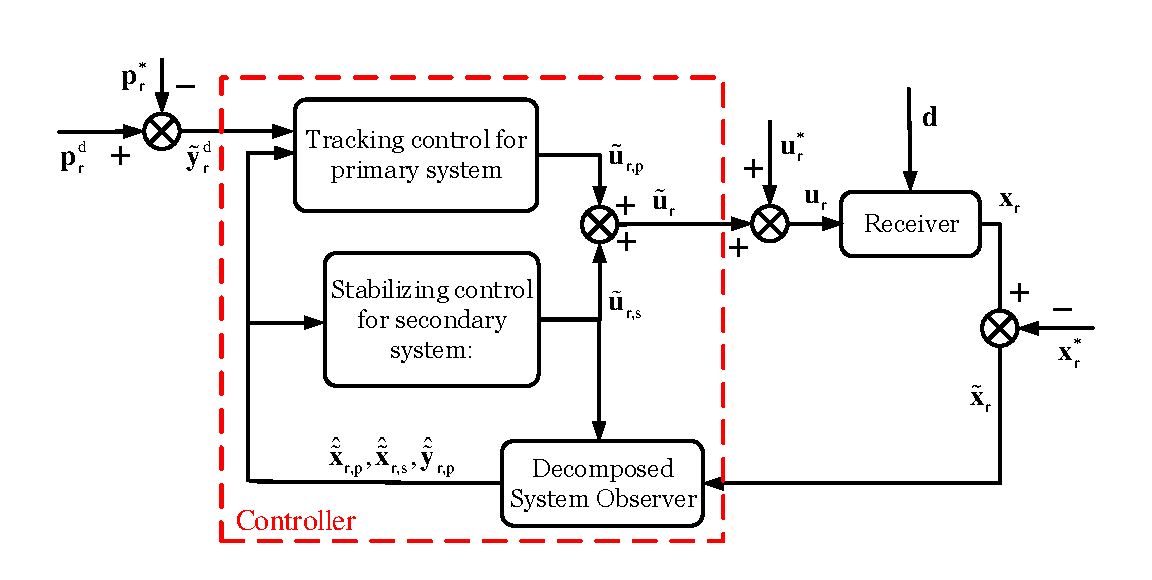
\includegraphics[
		width=12cm]{Figures/Figs_Ch7/Fig_CLSystem.eps}
	\end{center}
	\caption{Structure of the closed-loop system with ASD-based control.}
	\label{Fig_CLSystem}
\end{figure}

\section{Simulation Studies}

\label{Simulations}

In this section, the feasibility and the performance of the proposed
ASD-based station-keeping controller are investigated through the simulation.

\subsection{Simulation configuration}

A MATLAB/SIMULINK-based simulation environment with a three-dimensional
virtual-reality display has been developed by the authors' research
laboratory to simulate the PDR. The detailed information about the modeling
procedure, model parameters, and simulation environment can refer to
previous works \cite{ren2019reliable}, \cite{wei2016drogue}.

In the simulation, the trim condition is the level and forward flight with
the height $h_{\text{t}}^{\text{g}}=3000$m $(9843$ft$)$ and the velocity $v_{%
	\text{t}}^{\text{g}}=120$m/s $(393.72$ft/s$),$ as shown in Fig.~\ref%
{Fig_Frames}. Controller parameters are set as follows.

\textit{Longitudinal-channel primary controller parameters:}%
\begin{eqnarray*}
	\mathbf{Q}_{\text{rlon}} &=&\text{diag}\left( 4,10,10,1,10,10,1,3\right) ,%
	\mathbf{R}_{\text{rlon}}=\text{diag}\left( 50,50\right)  \\
	\mathbf{K}_{\mathbf{x}\text{1on}} &=&\left[
	\begin{array}{cccccc}
		0.6690 & 0.1816 & 72.926 & 1.3386 & -75.589 & 1.0669 \\
		0.0974 & -0.7903 & -354.56 & 0.0628 & 246.25 & -50.082%
	\end{array}%
	\right] ,\mathbf{K}_{\mathbf{e}\text{1on}}=\left[
	\begin{array}{cc}
		0.1392 & 0.0433 \\
		0.0250 & -0.2411%
	\end{array}%
	\right]
\end{eqnarray*}

\textit{Longitudinal-channel secondary controller parameters:}%
\begin{equation*}
\mathbf{C}_{\text{s1on}}=\left[
\begin{array}{cccccc}
-14.068 & 196.526 & 143428.581 & 2406.307 & -147654.857 & 2428.098 \\
194.075 & 76.508 & 44066.609 & 904.369 & -48027.709 & -41.490%
\end{array}%
\right] ,\mathbf{K}_{\text{rlon}}=\left[
\begin{array}{cc}
1 & 0 \\
0 & 1%
\end{array}%
\right]
\end{equation*}

\textit{Lateral-channel primary controller parameters:}%
\begin{eqnarray*}
	\mathbf{Q}_{\text{rlat}} &=&\text{diag}\left( 10,2,4,4,2,2,4\right) ,\mathbf{%
		R}_{\text{rlat}}=\text{diag}\left( 50,50\right)  \\
	\mathbf{K}_{\mathbf{x}\text{lat}} &=&\left[
	\begin{array}{cccccc}
		-0.3833 & 9.6773 & -287.58 & -250.74 & -5.7648 & -34.536 \\
		-0.0867 & 2.1597 & -70.513 & -61.301 & -1.4822 & -8.9008%
	\end{array}%
	\right] ,\mathbf{K}_{\mathbf{e}\text{lat}}=\left[
	\begin{array}{c}
		-0.0876 \\
		-0.0180%
	\end{array}%
	\right]
\end{eqnarray*}

\textit{Lateral-channel secondary controller parameters:}%
\begin{equation*}
\mathbf{C}_{\text{slat}}=\left[
\begin{array}{cccccc}
-1.272 & 55.046 & -880.467 & -775.037 & -7.652 & -52.170 \\
-0.143 & 9.216 & -173.189 & -149.751 & -1.826 & -13.936%
\end{array}%
\right] ,\mathbf{K}_{\text{rlat}}=\left[
\begin{array}{cc}
1 & 0 \\
0 & 1%
\end{array}%
\right]
\end{equation*}

\subsection{Simulation results}

\subsubsection{Station-keeping with constant mass}

In the first group of simulations, the joining phase from the standby point $%
A$ to the observation position $B$ and the pre-refueling phase from $B$ to
the pre-contact point $C$ are studied. During these phases, the receiver
mass remains unchanged. The position $A$ is set as $\mathbf{p}_{\text{r}0}^{%
	\text{t}}=\left[
\begin{array}{ccc}
-60 & -50 & 5%
\end{array}%
\right] ^{\text{T}}$, the position $B$ is set as $\mathbf{p}_{\text{r}1}^{%
	\text{t}}=\left[
\begin{array}{ccc}
-10 & -50 & 5%
\end{array}%
\right] ^{\text{T}}$, and the position $C$ is set as $\mathbf{p}_{\text{r}%
	2}^{\text{t}}=\left[
\begin{array}{ccc}
-25 & 0 & 5%
\end{array}%
\right] ^{\text{T}}$ in the tanker frame. The total simulation time is $%
T=200 $s. The first phase from $A$ to $B$ begins when $t=10$s, and the
second phase from $B$ to $C$ begins when $t=90$s. First, when the tanker
vortex is considered, the tracking response is presented in Fig.~\ref%
{Fig_TrackingResponse}. During the beginning $10$s, the receiver stays
relatively still to the tanker. Then, the receiver moves forward slowly, and
reaches the observation position $B$ at about $75$s. After staying still for
$15$s, the receiver begins to move backward\ and to the right to approach $C$%
, and gets there at about $160$s. It can also be seen that, during the whole
flight, the receiver tracks the reference trajectory well. The actual flight
trajectory is smooth, and the steady-state error is zero. The corresponding control inputs including the thrust and the actuator deflection are displayed in Fig.~\ref{Fig_Input}. Other nine states are displayed in Fig.~\ref{Fig_State}. They all meet the control requirements. Then, taking the atmospheric turbulence into consideration, the tracking response is presented
in Fig.~\ref{Fig_TrackingResponse1}. The maximum velocity of the
induced wind field by the atmospheric turbulence can reach 1m/s. Under this
circumstance, the receiver tracks the reference trajectory under slight
fluctuation. The whole tracking effect is satisfactory. Thus, the designed
controller can achieve good control effect in the presence of the wind
disturbances.
\begin{figure}[tph]
	\begin{center}
		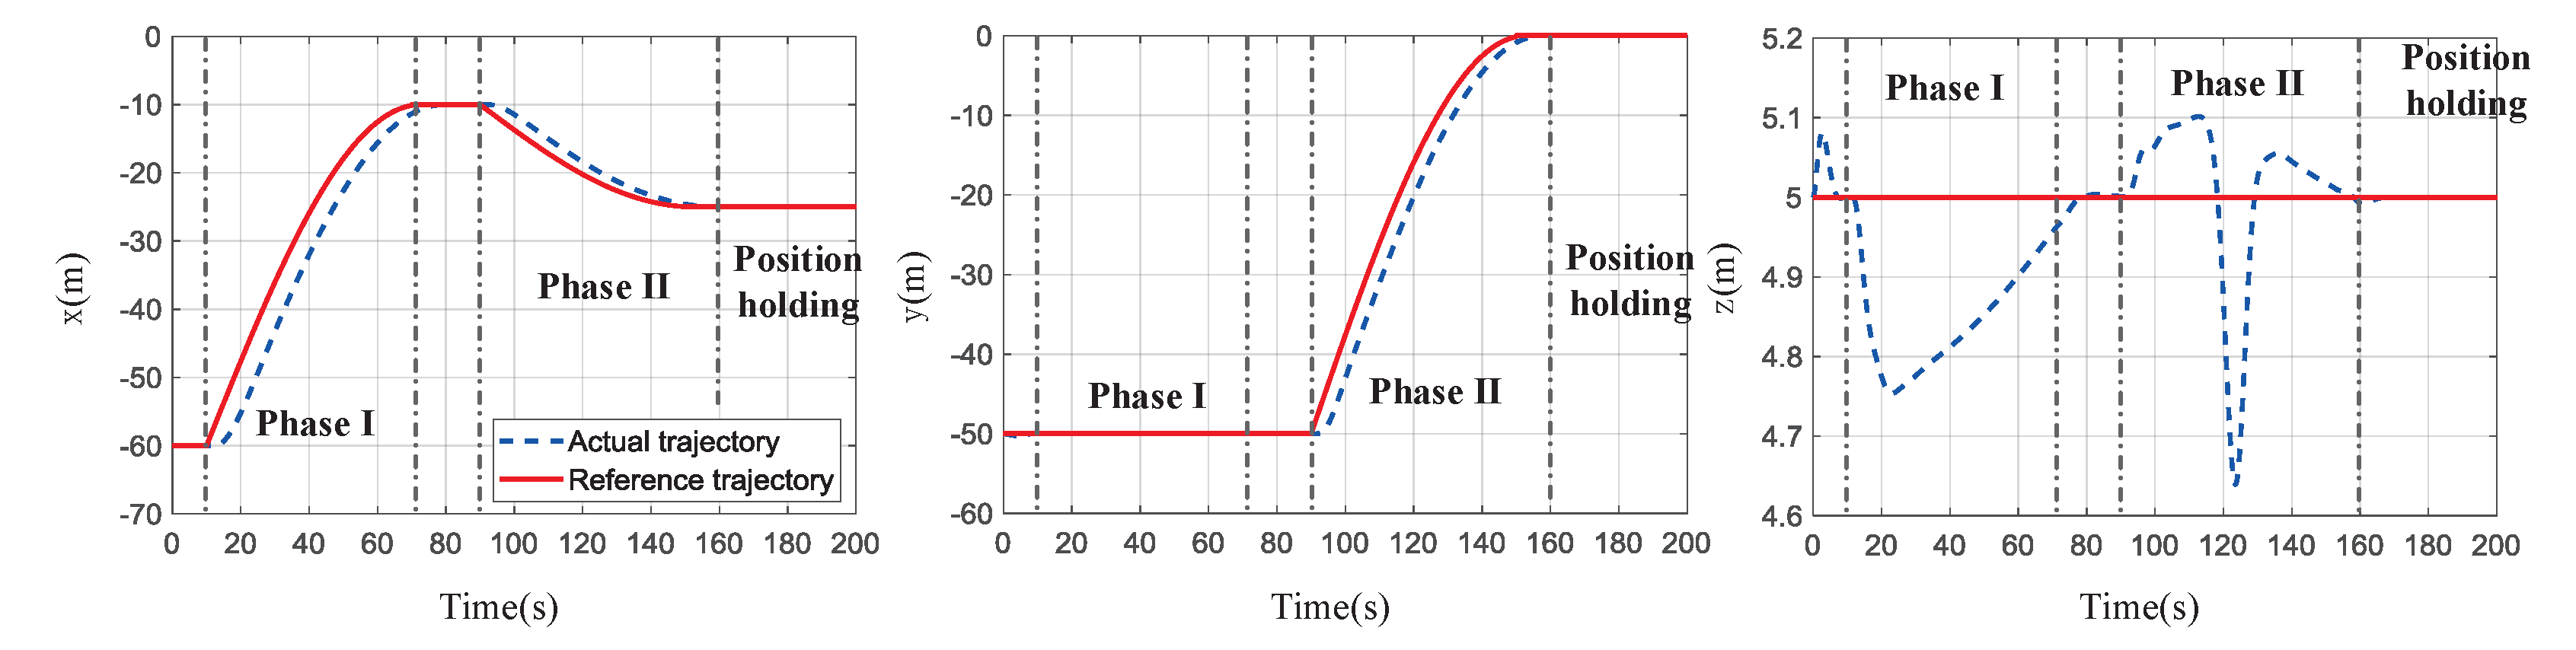
\includegraphics[scale=0.28]{Figures/Figs_Ch7/Fig_TrackingResponse.eps}
	\end{center}
	\caption{Trajectory tracking response under the tanker vortex.}
	\label{Fig_TrackingResponse}
\end{figure}
\begin{figure}[tph]
	\begin{center}
		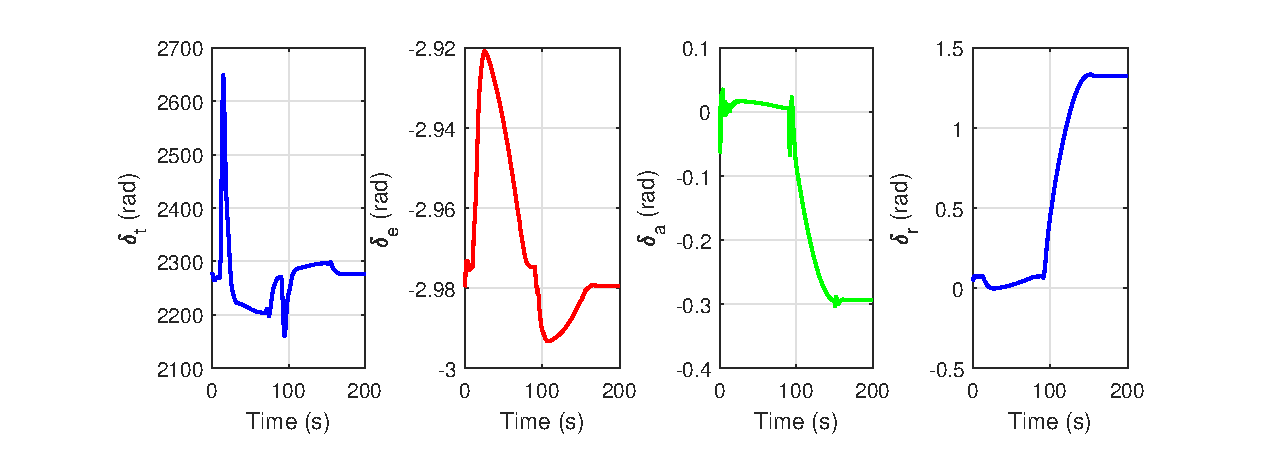
\includegraphics[scale=0.7]{Figures/Figs_Ch7/Fig_ActuatorInputs.eps}
	\end{center}
	\caption{Control inputs.}
	\label{Fig_Input}
\end{figure}
\begin{figure}[tph]
	\begin{center}
		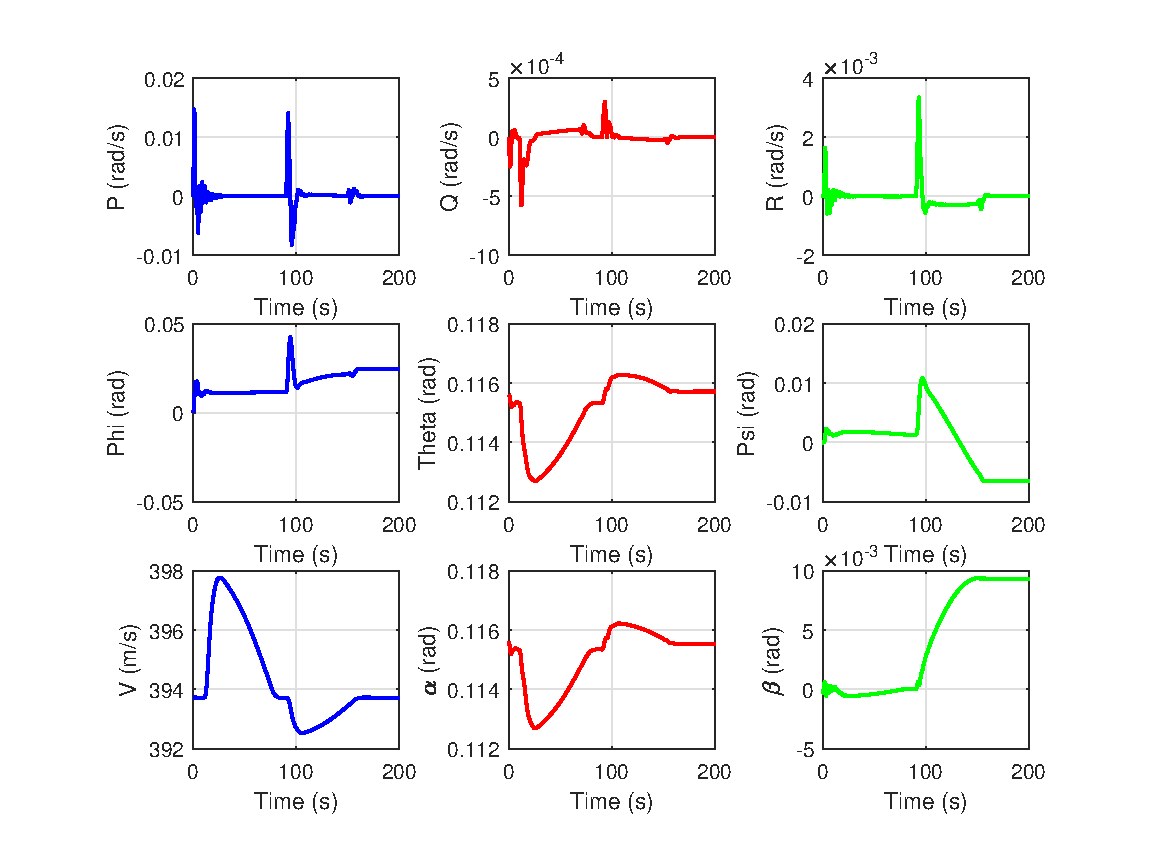
\includegraphics[scale=0.7]{Figures/Figs_Ch7/Fig_State9.eps}
	\end{center}
	\caption{State response.}
	\label{Fig_State}
\end{figure}
\begin{figure}[tph]
	\begin{center}
		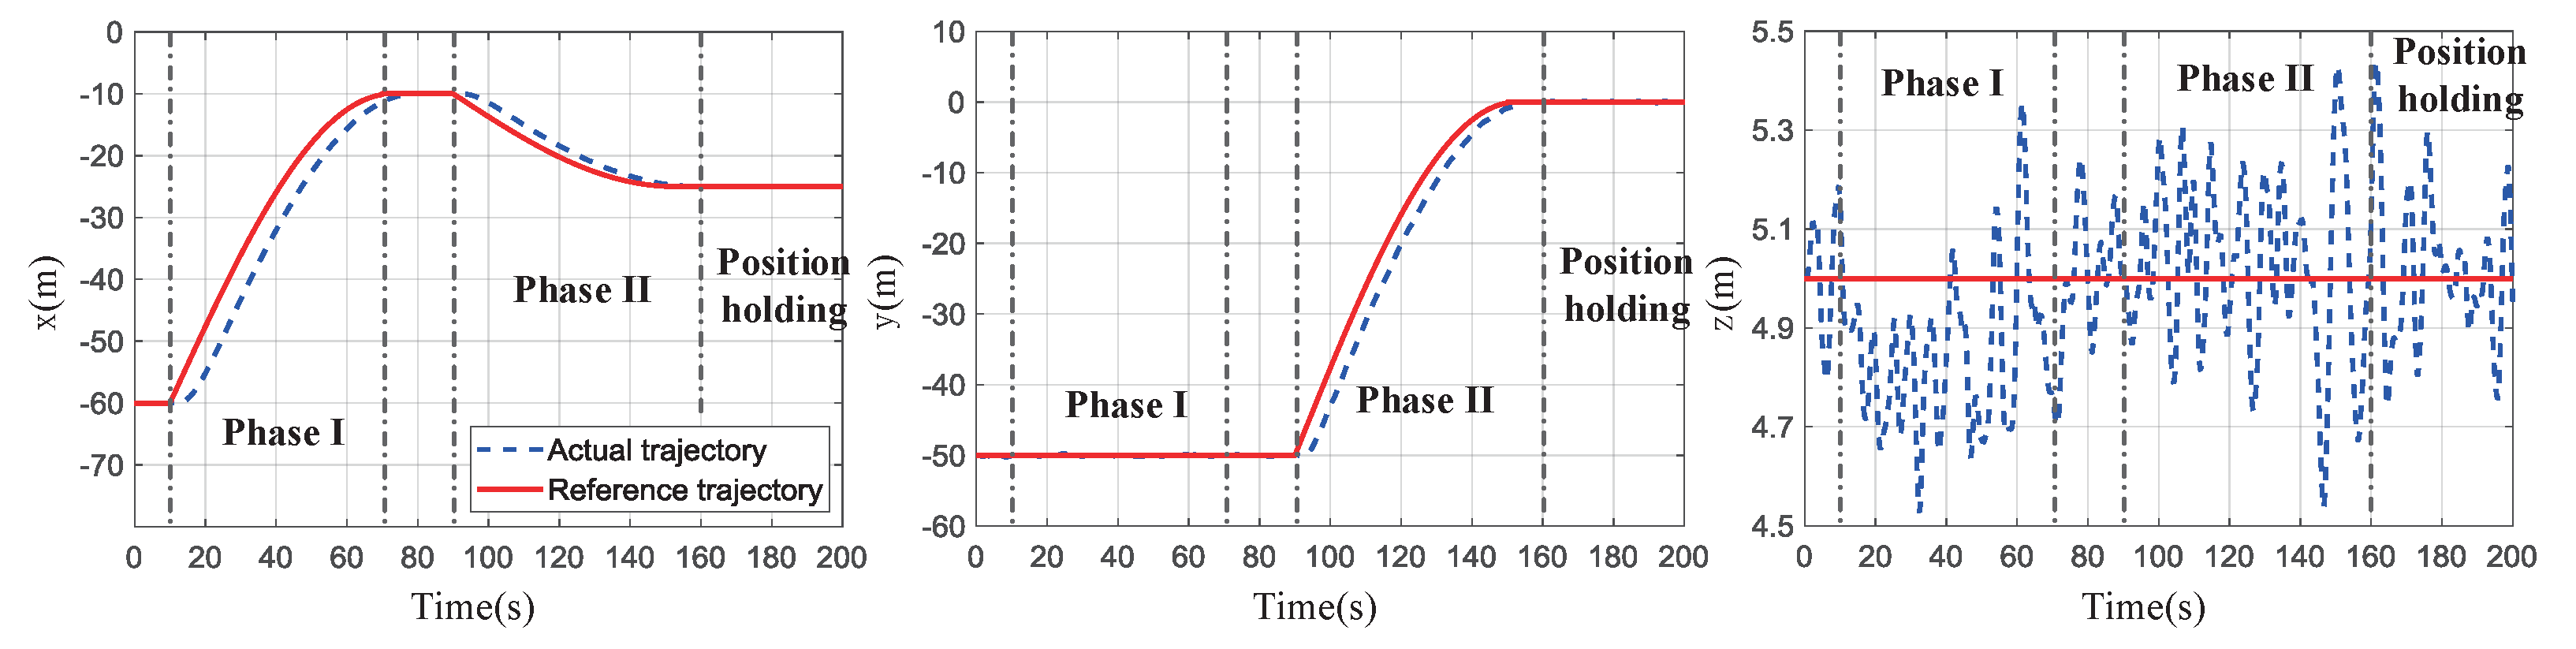
\includegraphics[scale=0.28]{Figures/Figs_Ch7/Fig_TrackingResponse1.eps}
	\end{center}
	\caption{Trajectory tracking response under the atmospheric turbulence.}
	\label{Fig_TrackingResponse1}
\end{figure}

\subsubsection{Station-keeping with varying mass}

In the second group of simulations, the fuel transferring phase, namely the
receiver and the tanker keep relatively stationary to transfer the fuel, is
considered. During this phase, the receiver mass increases gradually as the
fuel transfers. The receiver mass before fuel transfer is $m_{0}=9295$kg,
and the receiver mass after fuel transfer is $m_{1}=11295$kg. Total $2000$kg
fuel is transferred. If the fuel transferring speed is $v_{\text{ft}}=\dot{m}%
=20$kg/s, then the fuelling time is $T_{\text{ft}}=100$s. Suppose that, in
the tanker frame, the reference position of the receiver is $\mathbf{p}_{%
	\text{d}}^{\text{t}}=\left[
\begin{array}{ccc}
-15 & 0 & 5%
\end{array}%
\right] ^{\text{T}}$. The position holding response is displayed in Fig.~\ref%
{Fig_PositionHold}. It can be seen that the mass-varying receiver holds in
the refueling position well and the response under varying mass is just
slightly different from the response under the constant mass. This means the
proposed controller has robustness against the receiver mass change.

\begin{figure}[tbp]
	\begin{center}
		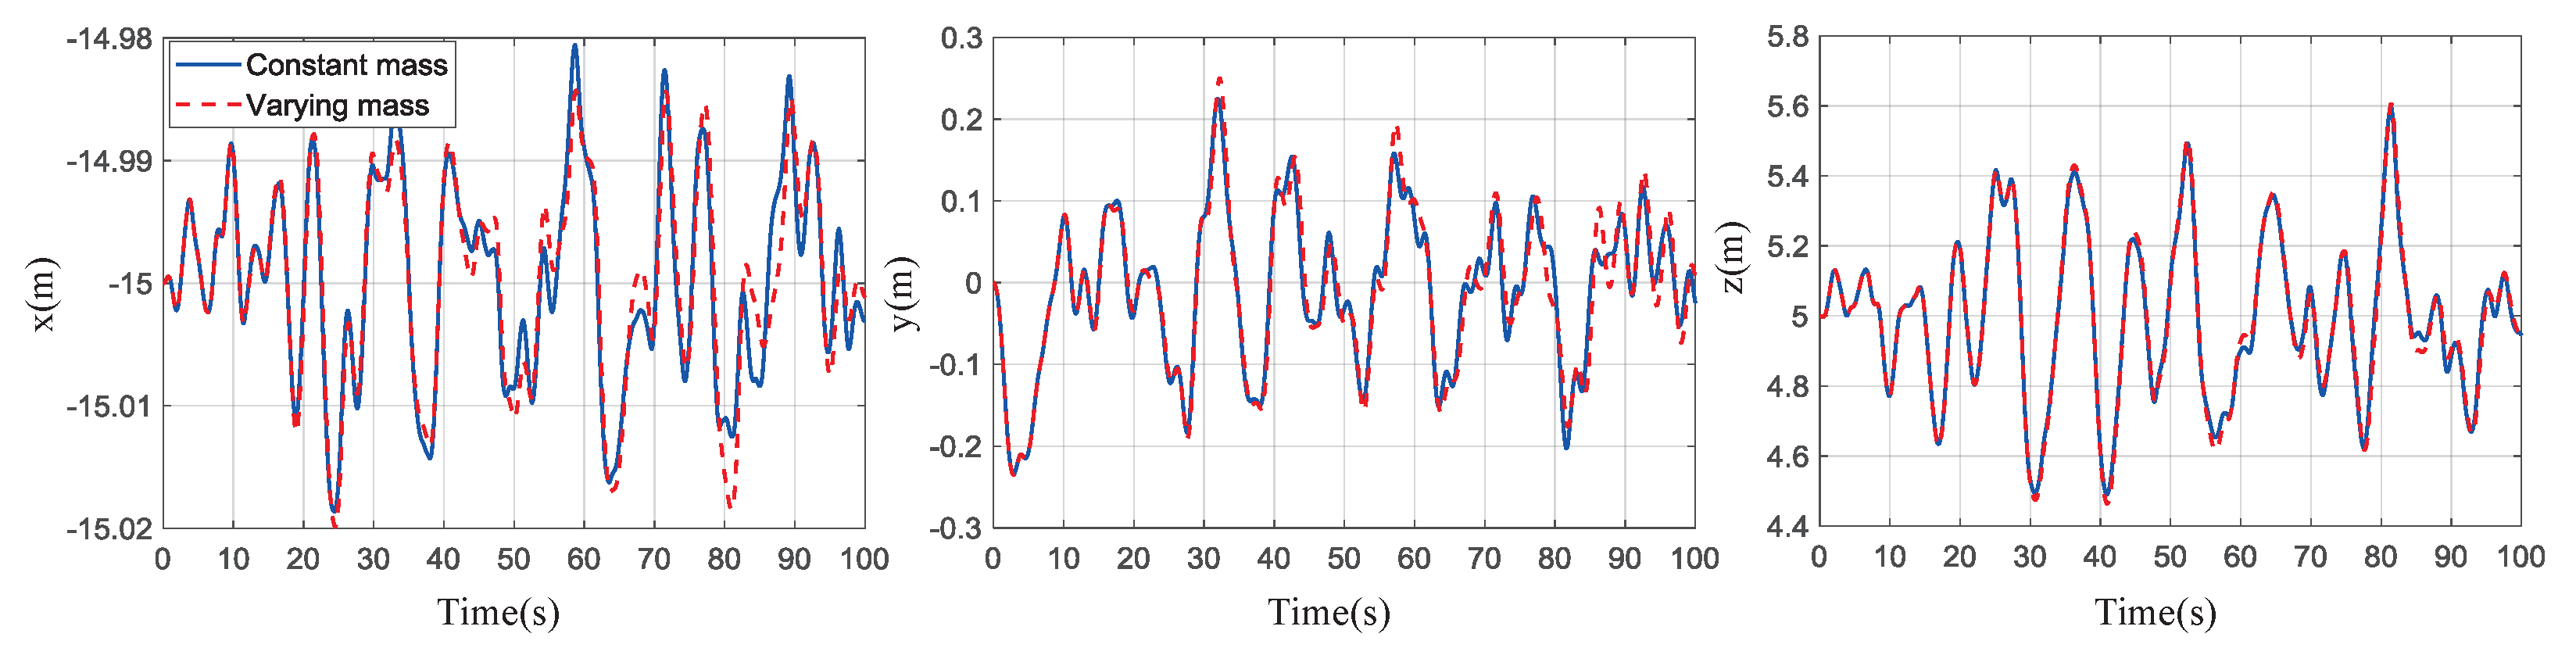
\includegraphics[scale=0.28]{Figures/Figs_Ch7/Fig_PositionHold.eps}
	\end{center}
	\caption{Position holding effect of the varying mass receiver.}
	\label{Fig_PositionHold}
\end{figure}

\section{Chapter Summary}

\label{Conclusions}

In this study, the station keeping problem for AAR has been addressed by an
ASD-based control method. In order to demonstrate its effectiveness, the
control method is applied to the PDR. Based on ASD, the original receiver
system is decomposed into a primary system and a secondary system. Through
designing a PI controller and a feedback linearization controller for these
two decomposed systems respectively, the final control input can be obtained
by combining these two controllers. Simulation results show that the
designed ASD-based station-keeping controller can satisfy the control
requirements of the trajectory tracking and position holding in the presence
of unknown disturbances and varying mass. While PI control and feedback
linearization control are not new, the salient feature of the proposed
control method lies in the fusion of them by using ASD to solve a
challenging nonlinear tracking problem. In future research, stability margin
could be introduced into the linear primary system to study the stability
and robustness of the full system in a more accurate and quantitative way.
Furthermore, frequency-domain compensation methods could be introduced into
the primary system to study the robustness performance improvement of the
full system.